\documentclass[12pt]{article}
\usepackage{setspace}
\doublespacing
\usepackage{caption}
\usepackage{tabularx}
\usepackage{booktabs}
\usepackage{adjustbox}
\usepackage{lipsum}
\newcolumntype{C}{>{\centering\arraybackslash}X}

% ============================================================
% METADATA
% ============================================================

\newcommand{\university}{COLUMBIA UNIVERSITY}
\newcommand{\department}{Department of Economics}

\newcommand{\classnum}{ECON UN3412}
\newcommand{\subject}{Introduction to Econometrics}
\newcommand{\semester}{Spring 2026}
\newcommand{\assignment}{Homework 7}

\newcommand{\instructors}{Seyhan Erden}
\newcommand{\instructoremail}{seyhan.erden@columbia.edu}

\newcommand{\name}{Tyler Sotomayor}
\newcommand{\email}{tyler.sotomayor@columbia.edu}

\newcommand{\duedate}{22 April 2026}

\newcommand{\sealfile}{ColumbiaSeal.png}
\newcommand{\sealsize}{0.22\textwidth}

\newcommand{\tathanksline}{Special thanks to the Teaching Assistants of \classnum}

% ============================================================
% TA LIST
% ============================================================

\newcommand{\TA}[2]{%
  {\large \textbf{#1}}\par
  \href{mailto:#2}{\texttt{#2}}\par
  \vspace{0.6cm}
}

\newcommand{\TAlist}{%
  \TA{Daniel Garcia}{dg3342@columbia.edu}
  \TA{Chris Kye}{mk4449@columbia.edu}
  \TA{Shivesh Babu Narayan}{sb5211@columbia.edu}
  \TA{Luca Salvatori}{ls4241@columbia.edu}
  \TA{Zijian Zhang}{zz3263@columbia.edu}
}

% ============================================================
% TITLE PAGE MACROS
% ============================================================

\newcommand{\maketitlepage}{%
\begin{titlepage}
\begingroup
\setlength{\parindent}{0pt}
\setlength{\parskip}{0.5em}
\centering

\vspace*{-0.8cm}
\includegraphics[width=\sealsize]{\sealfile}\par
\vspace{0.3cm}
{\LARGE \textbf{\university}}\par
{\large \department}

\vspace{1.1cm}

{\normalsize \textit{Completed in Partial Fulfillment of the Requirements of}}\par
\vspace{0.45cm}
{\Large \textbf{\classnum}}\par
{\Large \textbf{\subject}}\par
\vspace{0.3cm}
{\Large \semester}\par

\vspace{1.5cm}
{\fontfamily{lmr}\selectfont\Large\scshape \assignment}\par

\vspace{1.5cm}

{\large \textbf{\instructors}}\par
\vspace{2pt}
\href{mailto:\instructoremail}{\texttt{\instructoremail}}\par

\vspace{1.0cm}

{\large \textbf{\name}}\par
\href{mailto:\email}{\texttt{\email}}\par

\vspace*{\stretch{1}}
\endgroup
\end{titlepage}
}

\newcommand{\maketapage}{%
\begin{titlepage}
\begingroup
\setlength{\parindent}{0pt}
\setlength{\parskip}{0.45em}
\centering

{\normalsize \tathanksline}\par
\vspace{1.2cm}

\TAlist

\vspace*{\stretch{1}}
\endgroup
\end{titlepage}
}

% ------------------------------------------------------------
% LOAD TYLER'S CUSTOM MACROS AND FORMATTING
% ------------------------------------------------------------
% Import the fullpage package to adjust page margins
\usepackage{fullpage}
\usepackage{tikz}
\usepackage{pgfplots}
\pgfplotsset{compat=1.18}
\usepackage{tikz,pgfplots,caption}
\usepackage{graphicx}
\usepackage{adjustbox}
\usepackage{multicol}
\usepackage{tabularx}
\usepackage{array}
\usepackage{needspace}
\usepackage{tikz}
\usetikzlibrary{shapes,decorations,arrows,calc,arrows.meta,fit,positioning}
\newcolumntype{L}{>{\raggedright\arraybackslash}X}
\usepackage{longtable}
\usepackage{dcolumn}
\usepackage{xurl} % allows urls to break nicely across lines (recommended)

% Import the enumitem package to customize lists
\usepackage{enumitem}

% Import various AMS (American Mathematical Society) packages for mathematical symbols and formatting
\usepackage{amsfonts, amssymb, amsmath, amsthm}

% Import the mathtools package for advanced math typesetting
\usepackage{mathtools}

%For tables
\usepackage{multirow}

% Configure hyperlinks in the PDF file (e.g., author name, title)
\usepackage[pdftex, pdfauthor={\name}, pdftitle={\classnum~\assignment}]{hyperref}

% Import the xcolor package with the 'dvipsnames' option to define additional colors
\usepackage[dvipsnames]{xcolor}

% Import additional math fonts
\usepackage{bbm}

% Allow inserting images into the document
\usepackage{graphicx}

% Import additional mathematical script fonts
\usepackage{mathrsfs}

% Allow including entire PDF pages
\usepackage{pdfpages}

% Enable flexible table column formatting
\usepackage{tabularx}

% Enable landscape orientation for pages
\usepackage{pdflscape}

% Improve table formatting with multi-line cells
\usepackage{makecell}

% Improve table design and formatting
\usepackage{booktabs}

% Import natbib for better citation handling
\usepackage{natbib}

% Customize captions for tables and figures
\usepackage{caption}

% Allow subfigures within figures
\usepackage{subcaption}

% Import physics package for easier notation of derivatives, vectors, etc.
\usepackage{physics}

% Import the tcolorbox package to create colored boxes (e.g., for solutions or notes)
\usepackage[many]{tcolorbox}

% Enable conditional text inclusion (e.g., for draft versions)
\usepackage{version}

% Enable conditional logic in LaTeX (used for macros)
\usepackage{ifthen}

% Strike through mathematical expressions
\usepackage{cancel}

% Import the listings package to format source code
\usepackage{listings}

% Use the Courier font for code listings
\usepackage{courier}

% Import TikZ for creating diagrams and illustrations
\usepackage{tikz}

% Import a package for drawing game theory diagrams
\usepackage{istgame}

% Allow better placement of floating figures and tables
\usepackage{float}

% Customize hyperlink colors (e.g., blue links)
\hypersetup{
	colorlinks=true,
	linkcolor=blue,
	filecolor=magenta,
	urlcolor=blue,
}

% Adjust paragraph formatting
\setlength{\parindent}{0mm}  % No indentation at the start of paragraphs
\setlength{\parskip}{2mm}    % Space between paragraphs

% Customize numbered lists: (a), (b), (c), etc.
\setlist[enumerate]{label=({\alph*})}

% Customize nested numbered lists: (i), (ii), (iii), etc.
\setlist[enumerate, 2]{label=({\roman*})}

% Allow equations to break across pages (level 1 means minimal breaks)
\allowdisplaybreaks[1]

% Define a macro to generate a problem set header
\newcommand{\psetheader}{
	\ifthenelse{\isundefined{\collaborators}}{ % Check if collaborators are specified
		\begin{center}
			{\setlength{\parindent}{0cm} \setlength{\parskip}{0mm}
				
				% Display course number, semester, and assignment title on the left, name on the right
				{\textbf{\classnum~\semester:~\assignment} \hfill \name}
				
				% Display subject and email, with email as a clickable link
				\subject \hfill \href{mailto:\email}{\tt \email}
				
				% Display instructor names and due date
				Instructor:~\instructors \hfill Due Date:~\duedate	
				
				% Horizontal rule (separator line)
				\hrulefill}
		\end{center}
	}{
		\begin{center}
			{\setlength{\parindent}{0cm} \setlength{\parskip}{0mm}
				
				% If collaborators exist, add them as a footnote
				{\textbf{\classnum~\semester:~\assignment} \hfill \name\footnote{Collaborator(s): \collaborators}}
				
				% Display subject and email
				\subject \hfill \href{mailto:\email}{\tt \email}
				
				% Display instructor names and due date
				Instructor(s):~\instructors \hfill Due Date:~\duedate	
				
				\hrulefill}
		\end{center}
	}
}

% Customize page numbering: include class number, assignment, and page number
\usepackage{fancyhdr}
\pagestyle{fancy}
\fancyhf{}
\lfoot{\classnum~\assignment}
\rfoot{\thepage}
\renewcommand{\headrulewidth}{0pt}
\renewcommand{\footrulewidth}{0pt}

% Define a macro to format point values for problems
\makeatletter
\def\points{\@ifnextchar[{\@with}{\@without}}
\def\@with[#1]#2{{\ifthenelse{\equal{#2}{1}}{{[1 point, #1]}}{{[#2 points, #1]}}}}
\def\@without#1{\ifthenelse{\equal{#1}{1}}{{[1 point]}}{{[#1 points]}}}
\makeatother

% ---------------------------------------
% Elegant Theorem Style (Academic / Journal)
% ---------------------------------------
\newcommand{\MRS}{\operatorname{MRS}}

\makeatletter
\newtheoremstyle{econ-thm}% name
  {6pt}% Space above
  {6pt}% Space below
  {\normalfont}% Body font
  {}% Indent
  {\bfseries}% Default head font (BOLD ONLY)
  {.}% Punctuation after theorem number
  {0.5em}% Space after theorem head
  {%
    \textbf{\thmname{#1}\thmnumber{ #2}.}% <-- LABEL: bold italic
    \ifx\thmnote\@empty
    \else\ \textbf{\thmnote{#3}}\fi% <-- NAME: bold only
  }% Head spec
\makeatother

\theoremstyle{econ-thm}
\newtheorem{theorem}{Theorem}
\newtheorem{lemma}{Lemma}
\newtheorem{corollary}{Corollary}
\newtheorem{proposition}{Proposition}
\newtheorem{definition}{Definition}



% Define an environment for problems (sets text color to black)
\newenvironment{problem}[1]{\color{black} #1}{}

% Define a solution box with a green border and automatic proof environment
\newenvironment{solution}{%
  \leavevmode
  \begin{tcolorbox}[
    breakable,
    colback=green!5!white,
    colframe=green!75!black,
    enhanced jigsaw,
    % ↓ ensure no first-line indent anywhere in the box
    before upper={\parindent0pt\relax \parskip2mm}%
  ]%
  \proof[\scshape Solution:] \mbox{}\par\noindent
}{%
  \renewcommand{\qedsymbol}{$\blacksquare$}%
  \endproof
  \end{tcolorbox}%
}

% Define a reflection environment with a gray box
\newenvironment{reflection}{\begin{tcolorbox}[breakable, colback=black!8!white,colframe=black!60!white, enhanced jigsaw, parbox = false]\textsc{Reflections:}}{\end{tcolorbox}}

% Define a custom QED symbol for proofs
\newcommand{\qedh}{\renewcommand{\qedsymbol}{$\blacksquare$}\qedhere}

% Define custom colors for syntax highlighting
\definecolor{mygreen}{rgb}{0,0.6,0}
\definecolor{mygray}{rgb}{0.5,0.5,0.5}
\definecolor{mymauve}{rgb}{0.58,0,0.82}

% Define Stata programming language syntax highlighting for listings
\lstdefinelanguage{Stata}{
	% Define categories of keywords for Stata commands
	morekeywords=[1]{regress, reg, summarize, sum, display, di, generate, gen, bysort, use, import, delimited, predict, quietly, probit, margins, test},
	% Define reserved words
	morekeywords=[2]{boolean, break, byte, case, catch, class, const, continue, delete, double, else, enum, export, float, function, if, int, local, long, matrix, namespace, new, numeric, NULL, operator, pointer, private, protected, public, return, scalar, short, static, string, struct, super, switch, template, this, throw, typedef, typename, union, unsigned, using, vector, virtual, void, volatile, while,},
	% Define comment styles for Stata code
	morecomment=[l]{//},
	morecomment=[s]{/*}{*/},
	sensitive=true,
}

% Set global options for code listings (e.g., font, line numbering)
\lstset{ 
	backgroundcolor=\color{white},  
	basicstyle=\footnotesize\ttfamily, 
	numbers=left,
	numberstyle=\tiny\color{mygray},  
	keywordstyle=\color{blue},  
	commentstyle=\color{mygreen},  
	stringstyle=\color{mymauve},  
	frame=single,  
	tabsize=2,
}


% Override link colors to black
\hypersetup{citecolor=black, linkcolor=black}

% ------------------------------------------------------------
% AUTO-GENERATED MACROS FROM ps7_ajr.do
% ------------------------------------------------------------
% Auto-generated by ps7_ajr.do; do not edit by hand.
\newcommand{\ajrcabsecond}{0.944}
\newcommand{\ajrcasesecond}{0.176}
\newcommand{\ajrcabfirst}{-0.607}
\newcommand{\ajrcasefirst}{0.150}
\newcommand{\ajrcaRsq}{0.270}
\newcommand{\ajrcaN}{  64}
\newcommand{\ajrcbbsecond}{0.996}
\newcommand{\ajrcbsesecond}{0.240}
\newcommand{\ajrcbbfirst}{-0.510}
\newcommand{\ajrcbsefirst}{0.165}
\newcommand{\ajrcbRsq}{0.296}
\newcommand{\ajrcbN}{  64}
\newcommand{\ajrccbsecond}{1.281}
\newcommand{\ajrccsesecond}{0.402}
\newcommand{\ajrccbfirst}{-0.391}
\newcommand{\ajrccsefirst}{0.149}
\newcommand{\ajrccRsq}{0.130}
\newcommand{\ajrccN}{  60}
\newcommand{\ajrcdbsecond}{1.212}
\newcommand{\ajrcdsesecond}{0.392}
\newcommand{\ajrcdbfirst}{-0.394}
\newcommand{\ajrcdsefirst}{0.166}
\newcommand{\ajrcdRsq}{0.130}
\newcommand{\ajrcdN}{  60}
\newcommand{\ajrcebsecond}{0.578}
\newcommand{\ajrcesesecond}{0.082}
\newcommand{\ajrcebfirst}{-1.210}
\newcommand{\ajrcesefirst}{0.201}
\newcommand{\ajrceRsq}{0.466}
\newcommand{\ajrceN}{  37}
\newcommand{\ajrcfbsecond}{0.576}
\newcommand{\ajrcfsesecond}{0.091}
\newcommand{\ajrcfbfirst}{-1.137}
\newcommand{\ajrcfsefirst}{0.217}
\newcommand{\ajrcfRsq}{0.473}
\newcommand{\ajrcfN}{  37}
\newcommand{\ajrcgbsecond}{0.982}
\newcommand{\ajrcgsesecond}{0.331}
\newcommand{\ajrcgbfirst}{-0.432}
\newcommand{\ajrcgsefirst}{0.192}
\newcommand{\ajrcgRsq}{0.304}
\newcommand{\ajrcgN}{  64}
\newcommand{\ajrchbsecond}{1.107}
\newcommand{\ajrchsesecond}{0.503}
\newcommand{\ajrchbfirst}{-0.340}
\newcommand{\ajrchsefirst}{0.197}
\newcommand{\ajrchRsq}{0.328}
\newcommand{\ajrchN}{  64}
\newcommand{\ajrcibsecond}{0.981}
\newcommand{\ajrcisesecond}{0.196}
\newcommand{\ajrcibfirst}{-0.629}
\newcommand{\ajrcisefirst}{0.151}
\newcommand{\ajrciRsq}{0.287}
\newcommand{\ajrciN}{  61}
\newcommand{\ajrcbbsecondlat}{-0.647}
\newcommand{\ajrcbsesecondlat}{1.227}
\newcommand{\ajrcbbfirstlat}{2.002}
\newcommand{\ajrcbsefirstlat}{1.369}
\newcommand{\ajrcdbsecondlat}{0.939}
\newcommand{\ajrcdsesecondlat}{1.191}
\newcommand{\ajrcdbfirstlat}{-0.106}
\newcommand{\ajrcdsefirstlat}{1.424}
\newcommand{\ajrcfbsecondlat}{0.038}
\newcommand{\ajrcfsesecondlat}{0.507}
\newcommand{\ajrcfbfirstlat}{0.990}
\newcommand{\ajrcfsefirstlat}{1.274}
\newcommand{\ajrchbsecondlat}{-1.178}
\newcommand{\ajrchsesecondlat}{1.792}
\newcommand{\ajrchbfirstlat}{2.009}
\newcommand{\ajrchsefirstlat}{1.496}
\newcommand{\ajrcgbsecondasia}{-0.924}
\newcommand{\ajrcgsesecondasia}{0.370}
\newcommand{\ajrcgbfirstasia}{0.333}
\newcommand{\ajrcgsefirstasia}{0.486}
\newcommand{\ajrcgbsecondafr}{-0.464}
\newcommand{\ajrcgsesecondafr}{0.313}
\newcommand{\ajrcgbfirstafr}{-0.269}
\newcommand{\ajrcgsefirstafr}{0.353}
\newcommand{\ajrcgbsecondoth}{-0.941}
\newcommand{\ajrcgsesecondoth}{0.912}
\newcommand{\ajrcgbfirstoth}{1.241}
\newcommand{\ajrcgsefirstoth}{0.773}
\newcommand{\ajrchbsecondasia}{-1.047}
\newcommand{\ajrchsesecondasia}{0.505}
\newcommand{\ajrchbfirstasia}{0.472}
\newcommand{\ajrchsefirstasia}{0.524}
\newcommand{\ajrchbsecondafr}{-0.437}
\newcommand{\ajrchsesecondafr}{0.377}
\newcommand{\ajrchbfirstafr}{-0.258}
\newcommand{\ajrchsefirstafr}{0.344}
\newcommand{\ajrchbsecondoth}{-0.990}
\newcommand{\ajrchsesecondoth}{1.059}
\newcommand{\ajrchbfirstoth}{1.062}
\newcommand{\ajrchsefirstoth}{0.775}
\newcommand{\ajrTSLSb}{ 0.9443}
\newcommand{\ajrCOVb}{ 0.9443}
\newcommand{\ajrRFb}{ 0.9443}
\newcommand{\ajrTSLSfb}{ 0.996}
\newcommand{\ajrTSLSfse}{ 0.240}
\newcommand{\ajrGMMfb}{ 0.996}
\newcommand{\ajrGMMfse}{ 0.240}
\newcommand{\ajrLIMLfb}{ 0.996}
\newcommand{\ajrLIMLfse}{ 0.240}

% Auto-generated by ps7_sw_ee.do; do not edit by hand.
\newcommand{\fertN}{  254,654}
\newcommand{\fertOLSb}{-5.3870}
\newcommand{\fertOLSse}{ 0.0871}
\newcommand{\fertFSb}{ 0.0675}
\newcommand{\fertFSse}{ 0.0019}
\newcommand{\fertFSF}{1238.2}
\newcommand{\fertIVb}{-6.3137}
\newcommand{\fertIVse}{ 1.2747}
\newcommand{\fertIVctrlb}{-5.8211}
\newcommand{\fertIVctrlse}{ 1.2464}
\newcommand{\fertFSctrlF}{1280.9}
\newcommand{\movN}{ 516}
\newcommand{\movAiF}{ 78.28}
\newcommand{\movAip}{0.0000}
\newcommand{\movAiiF}{ 58.57}
\newcommand{\movAiip}{0.0000}
\newcommand{\movBbv}{-0.00317}
\newcommand{\movBsev}{ 0.00101}
\newcommand{\movBbm}{-0.00314}
\newcommand{\movBsem}{ 0.00070}
\newcommand{\movBbn}{-0.00211}
\newcommand{\movBsen}{ 0.00074}
\newcommand{\movBpvm}{0.9698}
\newcommand{\movBpvn}{0.2021}
\newcommand{\movBFj}{  6.80}
\newcommand{\movBpj}{0.0002}
\newcommand{\movBpredict}{-0.0106}
\newcommand{\movBpredSE}{ 0.0050}
\newcommand{\movBpredLo}{-0.0205}
\newcommand{\movBpredHi}{-0.0008}
\newcommand{\movCbv}{-0.00387}
\newcommand{\movCsev}{ 0.00098}
\newcommand{\movCbm}{-0.00389}
\newcommand{\movCsem}{ 0.00076}
\newcommand{\movCbn}{-0.00272}
\newcommand{\movCsen}{ 0.00077}
\newcommand{\movCpvm}{0.9811}
\newcommand{\movCpvn}{0.1781}
\newcommand{\movCpredict}{-0.0127}
\newcommand{\movCpredSE}{ 0.0048}
\newcommand{\movCpredLo}{-0.0222}
\newcommand{\movCpredHi}{-0.0032}
\newcommand{\movCFv}{ 847.1}
\newcommand{\movCFm}{ 848.1}
\newcommand{\movCFn}{ 729.0}
\newcommand{\movDbv}{-0.00317}
\newcommand{\movDsev}{ 0.00195}
\newcommand{\movDbm}{-0.00412}
\newcommand{\movDsem}{ 0.00129}
\newcommand{\movDbn}{-0.00258}
\newcommand{\movDsen}{ 0.00177}
\newcommand{\movDpredict}{-0.0082}
\newcommand{\movDpredSE}{ 0.0089}
\newcommand{\movEJ}{  8.14}
\newcommand{\movEJdf}{ 6}
\newcommand{\movEJp}{0.2279}
\newcommand{\namesN}{ 4870}
\newcommand{\namesCBoverall}{ 0.0805}
\newcommand{\namesCBwhite}{ 0.0965}
\newcommand{\namesCBblack}{ 0.0645}
\newcommand{\namesNwhite}{ 2435}
\newcommand{\namesNblack}{ 2435}
\newcommand{\namesDiff}{ 0.0320}
\newcommand{\namesSEdiff}{ 0.0078}
\newcommand{\namesT}{  4.12}
\newcommand{\namesCIlo}{ 0.0168}
\newcommand{\namesCIhi}{ 0.0473}
\newcommand{\namesLPMb}{-0.0320}
\newcommand{\namesLPMse}{ 0.0078}
\newcommand{\namesBblackB}{-0.0304}
\newcommand{\namesBblackSE}{ 0.0155}
\newcommand{\namesBfemB}{ 0.0102}
\newcommand{\namesBfemSE}{ 0.0137}
\newcommand{\namesBbfemB}{-0.0022}
\newcommand{\namesBbfemSE}{ 0.0179}
\newcommand{\namesMaleb}{-0.0304}
\newcommand{\namesMalese}{ 0.0155}
\newcommand{\namesFemb}{-0.0326}
\newcommand{\namesFemse}{ 0.0090}
\newcommand{\namesGenPint}{0.9006}
\newcommand{\namesHiLo}{ 0.0141}
\newcommand{\namesHiLose}{ 0.0078}
\newcommand{\namesCblackB}{-0.0231}
\newcommand{\namesCblackSE}{ 0.0106}
\newcommand{\namesChighB}{ 0.0229}
\newcommand{\namesChighSE}{ 0.0120}
\newcommand{\namesCbhighB}{-0.0178}
\newcommand{\namesCbhighSE}{ 0.0156}
\newcommand{\namesWhHi}{ 0.1079}
\newcommand{\namesWhLo}{ 0.0850}
\newcommand{\namesWhHiLo}{ 0.0229}
\newcommand{\namesBlHi}{ 0.0670}
\newcommand{\namesBlLo}{ 0.0619}
\newcommand{\namesBlHiLo}{ 0.0052}
\newcommand{\namesHiLoRacePint}{0.2532}
\newcommand{\namesRandF}{  0.69}
\newcommand{\namesRandp}{0.7353}


\begin{document}

\pagenumbering{gobble}
\maketitlepage
\maketapage

\clearpage
\pagenumbering{roman}
\tableofcontents
\clearpage
\pagenumbering{arabic}
\psetheader

% ============================================================
% PROBLEM 1 -- AJR 2001 IV/TSLS  (GRADED, 60 POINTS)
%   Problem statements reproduced verbatim from ps7_spring 2026.pdf.
% ============================================================

\section*{Problem 1 \points{60}}
\addcontentsline{toc}{section}{Problem 1: Acemoglu--Johnson--Robinson (2001) IV/TSLS Replication}

\begin{problem}
Students who are interested in development economics may be familiar with the work of Daron Acemoglu. A seminal work in the field that this question will be drawing from is:

Acemoglu, D, Johnson, S, Robinson, J, \textit{The Colonial Origins of Comparative Development: An Empirical Investigation}, The American Economic Review, Vol 91, No. 5, Dec. 2001, pp. 1369--1401.

In this paper the authors seek to further the understanding of why countries farther from the equator seem to enjoy higher economic growth. They attribute the difference to a pattern of European colonization which was different in different climates. Areas in which Europeans had more resistance to the local diseases were colonized such that governmental institutions came to resemble those in Europe. Areas where Europeans had less resistance to the local diseases were colonized such that governmental institutions were created to extract wealth from the colony and its local inhabitants.

The authors have assessments of current government institutions in many countries, and of the government institutions that existed in the past, and data on GDP. They would like to show that government institutions are a large factor in determining economic well-being. They also would like to show that due to the extraordinarily high persistence of culture, current institutions seem to have their roots in the distant past, particularly the in the experience of European colonization. Economists sometimes use the word strong to indicate democratic-type institutions and the word weak to indicate institutions that do not offer much protection from rights violations and expropriation.

But the authors worry about endogeneity. As an example, the colonists' wealth could feed back into their choice of government institutions. If that is true, then it is some aspect of colonization other than disease resistance that may have caused the path-dependent outcome of institutions. Or it may have been the religion or some other aspect of the culture of particular European groups that caused different paths for institutions.

Instrumental variables and two-stage least squares provide a mechanism to examine only the input of European disease resistance during the colonization period on the formulation of governmental institutions. The governmental institutions index is regressed upon the European mortality rate during colonization, and control variables. The predicted governmental institutions strength can then be interpreted as the portion of institutional strength that can be attributed to the European disease resistance. The outcome of these regressions is quite interesting on its own, and the authors always report both stages of their two-stage process.

The predicted institutional strength is then regressed on GDP to show that past European disease resistance is a major factor in explaining the current arrangement of GDP around the world, and the linkage between the past experience and the current situation is governmental institutions. Prof.\ Acemoglu provides the data, and the Stata do files, for this paper on his website.

Despite a quick mention of clustered standard errors within climate groups in footnote 18, the authors run and report their results without using robust standard errors. In this question you will replicate some of the results using robust standard errors, and re-assess the statistical significance and the conclusions. The paper is an interesting and accessible read about both instrumental variables and economic development.

For this question, supply your written answers and Stata output sections as usual. Also submit your Stata do file as the last part of the question. The first grouping of TSLS results are reported in table 4 in the paper, page 1386, reprinted below.

Open the dataset and look at the variables. The authors' ultimate goal is to predict log 1995 GDP, \textit{logpgp95}, what we would call $Y$ using Stock and Watson terminology. The instrument, the $Z$ variable, is \textit{logem4}, the log of the colonial settler mortality rate. The instrumented variable, the $X$, will be \textit{avexpr}, the average (contemporary) protection against expropriation risk, an index value. The only exogenous variable, $W$, in the any of the first six regressions is a measure of the latitude, \textit{lat\_abst}. Use the \textit{ivregress} command with the \textit{2sls} estimation methodology. For options use both \textit{vce(robust)} and ``\textit{first}'', in order to see the first stage results also.

Panel C in table 4 are the OLS regressions of \textit{logpgp95} on \textit{avexpr}. No need to recreate these because the focus of this problem set is IV and TSLS. The authors show these OLS results for the sake of comparison, and note that the estimated coefficient of interest is larger when estimated using IV.
\end{problem}

\begin{enumerate}

% =================== PART (a) ===================
\item
\begin{problem}{\points{10}}
First a preliminary step. The dataset includes countries that do not have a European colonial history, or that are missing substantive data pieces. The authors have coded the useable countries with a one in the variable ``\textit{baseco}.'' Use the ``\textit{keep}'' command to keep only the observations that have this coding.

Run the TSLS model in table 4, regression 1. Your estimated coefficients should match the authors. Compare all the standard errors, first stage and second stage, in your results to the ones published. Take note in your mind for later of any differences greater than 0.2 in standard errors between your results and the authors'. Run the model for regression 2, which adds the exogenous variable of \textit{lat\_abst}. Again, compare your standard errors and the authors. After providing your Stata commands and output, so at the end of your answer to this question part, part (a), communicate to your graders which standard errors, if any, deviated by more than 0.2 when using the robust option. (Include the first stage regressions and standard errors in your review.)
\end{problem}
\begin{solution}
After restricting to \texttt{baseco == 1} ($n = 64$), the two TSLS specifications are
\begin{align*}
\text{(1)}\quad \log\text{GDPpc}_{95,i} &= \beta_0 + \beta_1\,\text{avexpr}_i + u_i, \\
\text{avexpr}_i &= \pi_0 + \pi_1\,\text{logem4}_i + v_i,
\end{align*}
and
\begin{align*}
\text{(2)}\quad \log\text{GDPpc}_{95,i} &= \beta_0 + \beta_1\,\text{avexpr}_i + \beta_2\,\text{lat\_abst}_i + u_i, \\
\text{avexpr}_i &= \pi_0 + \pi_1\,\text{logem4}_i + \pi_2\,\text{lat\_abst}_i + v_i.
\end{align*}
The Stata calls (shown with the condensed output) are
\begin{lstlisting}[language=Stata,basicstyle=\footnotesize\ttfamily,breaklines=true]
use "data/maketable4.dta", clear
keep if baseco == 1
* Regression 1
ivregress 2sls logpgp95 (avexpr = logem4), vce(robust) first
* Regression 2
ivregress 2sls logpgp95 lat_abst (avexpr = logem4), vce(robust) first
\end{lstlisting}
The second-stage coefficients on \texttt{avexpr} are $\hat{\beta}_1 = \ajrcabsecond$ (col.\ 1) and $\ajrcbbsecond$ (col.\ 2), which round to the authors' reported $0.94$ and $1.00$. The first-stage coefficients on \texttt{logem4} are $\ajrcabfirst$ (col.\ 1) and $\ajrcbbfirst$ (col.\ 2), which match the authors' $-0.61$ and $-0.51$ up to rounding. Columns (1) and (2) of Table~\ref{tab:ajr-table4} in the Appendix collect the coefficient and standard-error pairs for easy side-by-side reading, and the SE comparison for the two regressions is summarised below with the paper's non-robust numbers in brackets.
\begin{center}
\begin{tabular}{l cc cc}
\toprule
                                   & \multicolumn{2}{c}{\textbf{Regression 1 (col.\ 1)}} & \multicolumn{2}{c}{\textbf{Regression 2 (col.\ 2)}} \\
\cmidrule(lr){2-3}\cmidrule(lr){4-5}
                                   & Paper SE & Robust SE & Paper SE & Robust SE \\ \midrule
2nd stage: \texttt{avexpr}         & 0.16     & \ajrcasesecond    & 0.22     & \ajrcbsesecond     \\
2nd stage: \texttt{lat\_abst}      & ---      & ---       & 1.34     & \ajrcbsesecondlat  \\
1st stage: \texttt{logem4}         & 0.13     & \ajrcasefirst     & 0.14     & \ajrcbsefirst      \\
1st stage: \texttt{lat\_abst}      & ---      & ---       & 1.34     & \ajrcbsefirstlat   \\
\bottomrule
\end{tabular}
\end{center}
\textbf{SE deviations $\boldsymbol{>}$ 0.2 for regressions 1 and 2.} None. On the variable of interest \texttt{avexpr}, the paper's $0.16$ and $0.22$ compare with my robust $\ajrcasesecond$ and $\ajrcbsesecond$---moves of $0.02$ in each case. The $\texttt{logem4}$ first-stage SEs move by at most $0.03$. The largest move anywhere in these two regressions is on the column~(2) \texttt{lat\_abst} second-stage SE (paper $1.34$ versus robust $\ajrcbsesecondlat$, a gap of $\approx 0.11$), still well under the $0.2$ threshold. The paper's non-robust SEs are within sampling noise of the robust ones, which is evidence that heteroskedasticity is not severe in the base-sample cross-section of 64 countries.
\end{solution}

% =================== PART (b) ===================
\item
\begin{problem}{\points{10}}
In class, we discussed the three methods of estimating the 2sls coefficients, namely \textit{TSLS} as you use it in (a), the \textit{covariance ratio formula} (see eq 12.4 in the textbook), and the \textit{reduced form equation}s approach. Using the dependent variable (i.e., \textit{logpgp95}) and the endogenous $X$-variable that needs to be instrumented (i.e., \textit{avexpr}) and the $Z$-instrumental variable (i.e., \textit{logem4}) as in the first part of (a), show that all the three methods would result in the same 2sls slope coefficient.
\end{problem}
\begin{solution}
Let $Y_i = \log\text{GDPpc}_{95,i}$, $X_i = \texttt{avexpr}_i$, and $Z_i = \texttt{logem4}_i$ on the base sample of $n=64$ countries. The three estimators I compute are
\begin{align*}
(\text{i})\;\;\hat{\beta}_1^{\text{TSLS}} &= \text{the ivregress 2sls coefficient}, \\
(\text{ii})\;\;\hat{\beta}_1^{\text{COV}} &= \frac{s_{ZY}}{s_{ZX}} = \frac{\tfrac{1}{n-1}\sum_i (Z_i-\bar Z)(Y_i-\bar Y)}{\tfrac{1}{n-1}\sum_i (Z_i-\bar Z)(X_i-\bar X)}, \\
(\text{iii})\;\;\hat{\beta}_1^{\text{RF}} &= \frac{\hat{\pi}_1^{Y}}{\hat{\pi}_1^{X}},
\end{align*}
where in (iii) $\hat{\pi}_1^{Y}$ is the OLS slope from regressing $Y$ on $Z$ and $\hat{\pi}_1^{X}$ is the OLS slope from regressing $X$ on $Z$.
Run in Stata:
\begin{lstlisting}[language=Stata,basicstyle=\footnotesize\ttfamily,breaklines=true]
* (i) TSLS
ivregress 2sls logpgp95 (avexpr = logem4), vce(robust)
* (ii) covariance ratio
sum logpgp95 if !missing(avexpr,logem4)
scalar ybar = r(mean)
sum avexpr if !missing(logpgp95,logem4)
scalar xbar = r(mean)
sum logem4 if !missing(logpgp95,avexpr)
scalar zbar = r(mean)
gen zy = (logem4 - zbar) * (logpgp95 - ybar)
gen zx = (logem4 - zbar) * (avexpr   - xbar)
sum zy if !missing(avexpr,logem4); scalar s_zy = r(mean)*(r(N)/(r(N)-1))
sum zx if !missing(avexpr,logem4); scalar s_zx = r(mean)*(r(N)/(r(N)-1))
display s_zy/s_zx
* (iii) reduced-form ratio
reg logpgp95 logem4 if !missing(avexpr)
scalar piY = _b[logem4]
reg avexpr   logem4 if !missing(logpgp95)
scalar piX = _b[logem4]
display piY/piX
drop zy zx
\end{lstlisting}
The three computations give
\[
\hat{\beta}_1^{\text{TSLS}} = \ajrTSLSb,
\qquad
\hat{\beta}_1^{\text{COV}}  = \ajrCOVb,
\qquad
\hat{\beta}_1^{\text{RF}}    = \ajrRFb,
\]
so numerically the three agree to every digit Stata prints, which is the equivalence the textbook promises. The algebraic reason is straightforward. In a just-identified model with one endogenous regressor $X$ and one instrument $Z$, the TSLS estimator can be written
\[
\hat{\beta}_1^{\text{TSLS}}
= \frac{\sum_i (\hat X_i - \bar{\hat X})(Y_i - \bar Y)}{\sum_i (\hat X_i - \bar{\hat X})^2},
\quad\text{where}\quad
\hat X_i = \hat{\pi}_0 + \hat{\pi}_1 Z_i.
\]
Since $\hat X_i - \bar{\hat X} = \hat{\pi}_1 (Z_i - \bar Z)$, the $\hat{\pi}_1$ cancels out of the numerator and ratio of squares, leaving
\[
\hat{\beta}_1^{\text{TSLS}}
= \frac{\sum_i (Z_i - \bar Z)(Y_i - \bar Y)}{\hat{\pi}_1 \sum_i (Z_i - \bar Z)^2}
= \frac{s_{ZY}/s_{ZZ}}{\hat{\pi}_1} = \frac{s_{ZY}/s_{ZZ}}{s_{ZX}/s_{ZZ}} = \frac{s_{ZY}}{s_{ZX}},
\]
which is exactly the covariance-ratio formula (Stock \& Watson eq.\ 12.4). For the same reason, $s_{ZY}/s_{ZZ}$ is the OLS slope $\hat{\pi}_1^{Y}$ from the reduced form $Y_i = \pi_0 + \pi_1^{Y} Z_i + \epsilon_i$, while $s_{ZX}/s_{ZZ}$ is the first-stage slope $\hat{\pi}_1^{X}$, so $\hat{\beta}_1^{\text{TSLS}} = \hat{\pi}_1^{Y}/\hat{\pi}_1^{X}$---the reduced-form ratio. The three formulas are therefore identical in finite samples, not merely asymptotically. This Wald-ratio representation is what makes the identification argument transparent: the instrument's effect on $Y$ is attributed entirely to its effect on $X$, rescaled by that effect.
\end{solution}

% =================== PART (c) ===================
\item
\begin{problem}{\points{8}}
Repeat the process for regressions 3 and 4 but without the four countries that are the standouts in terms of GDP, US, Canada, Australia, and New Zealand. The dummy variable coded to 1 is called \textit{rich4}. To exclude these four countries, add the clause ``\textit{if rich4 !=1}'' to your command after your other variables but before your comma for the options. Again note any differences in standard errors greater than 0.2 in absolute value.

Repeat for regressions 5 and 6, this time excluding observations having the variable ``\textit{africa}'' coded as one. (The rich 4 should be back in the data being used in the regression.) Make sure that your resulting coefficient estimates match the authors'. Note SE differences beyond 0.2.

After providing your Stata commands and output, so at the end, communicate to your graders which standard errors, if any, deviated by more than 0.2 when using the robust option. (Include first stage regressions and standard errors in your review.)
\end{problem}
\begin{solution}
The four specifications are
\begin{lstlisting}[language=Stata,basicstyle=\footnotesize\ttfamily,breaklines=true]
* Regression 3: base without Neo-Europes (rich4)
ivregress 2sls logpgp95 (avexpr = logem4)          if rich4!=1, vce(robust) first
* Regression 4: base without Neo-Europes + lat_abst
ivregress 2sls logpgp95 lat_abst (avexpr = logem4) if rich4!=1, vce(robust) first
* Regression 5: base without Africa
ivregress 2sls logpgp95 (avexpr = logem4)          if africa!=1, vce(robust) first
* Regression 6: base without Africa + lat_abst
ivregress 2sls logpgp95 lat_abst (avexpr = logem4) if africa!=1, vce(robust) first
\end{lstlisting}
The resulting second-stage coefficients on \texttt{avexpr} are $\ajrccbsecond$, $\ajrcdbsecond$, $\ajrcebsecond$, and $\ajrcfbsecond$, matching the authors' $1.28$, $1.21$, $0.58$, $0.58$ to the second decimal. Dropping the four Neo-Europes \emph{raises} the estimated institutions effect from roughly one to roughly $1.2$--$1.3$, consistent with the paper's interpretation that the Neo-Europes (US, Canada, Australia, New Zealand) pull the fitted line slightly flatter because their exceptional GDP is not fully proportional to their institutional quality. Dropping Africa, by contrast, more than halves the estimated effect to $\approx 0.58$: without the large institutional-to-GDP gap between Sub-Saharan Africa and the rest of the ex-colonial world, the slope falls sharply even though the first-stage logem4 coefficient doubles in absolute value (\texttt{logem4}: $\ajrcebfirst$ in column 5 versus $\ajrcabfirst$ in column 1), reflecting the fact that African mortality rates were exceptional.

The full Table~\ref{tab:ajr-table4} collects these columns, and the SE comparison is:
\begin{center}
\footnotesize
\setlength{\tabcolsep}{4pt}
\begin{tabular}{l cccc cccc}
\toprule
                                   & \multicolumn{4}{c}{\textbf{No Neo-Europes} (cols.\ 3 \& 4)} & \multicolumn{4}{c}{\textbf{No Africa} (cols.\ 5 \& 6)} \\
\cmidrule(lr){2-5}\cmidrule(lr){6-9}
                                   & Pap 3 & Rob 3 & Pap 4 & Rob 4 & Pap 5 & Rob 5 & Pap 6 & Rob 6 \\ \midrule
2nd: \texttt{avexpr}               & 0.36  & \ajrccsesecond  & 0.35 & \ajrcdsesecond & 0.10 & \ajrcesesecond & 0.12 & \ajrcfsesecond \\
2nd: \texttt{lat\_abst}            & ---   & ---     & 1.46 & \ajrcdsesecondlat & --- & ---   & 0.84 & \ajrcfsesecondlat \\
1st: \texttt{logem4}               & 0.13  & \ajrccsefirst   & 0.14 & \ajrcdsefirst  & 0.22 & \ajrcesefirst  & 0.24 & \ajrcfsefirst  \\
1st: \texttt{lat\_abst}            & ---   & ---     & 1.50 & \ajrcdsefirstlat & --- & ---   & 1.43 & \ajrcfsefirstlat \\
\bottomrule
\end{tabular}
\end{center}
\textbf{SE deviations $\boldsymbol{>}$ 0.2 for regressions 3--6.} None in the \texttt{avexpr} or \texttt{logem4} rows (largest gap $\approx 0.04$). \emph{Two} of the second-stage \texttt{lat\_abst} SEs do cross the threshold, however: in column~(4) the paper's $1.46$ becomes $\ajrcdsesecondlat$ under robust inference (a move of $\approx 0.27$), and in column~(6) the paper's $0.84$ becomes $\ajrcfsesecondlat$ (a move of $\approx 0.33$). In the first-stage, the \texttt{lat\_abst} SEs are $\ajrcdsefirstlat$ and $\ajrcfsefirstlat$ versus $1.50$ and $1.43$---both moves are small. The take-away is the same as in (a): the two-stage results on the variable of interest, \texttt{avexpr}, are robust to swapping in Huber--White SEs; both larger moves I observe are on an auxiliary latitude control whose own coefficient is statistically indistinguishable from zero in either regression.
\end{solution}

% =================== PART (d) ===================
\item
\begin{problem}{\points{8}}
For regressions 7 and 8 do not exclude the rich4 or africa. As control variables, $W$, the goal is to use continent indicators. The continent indicators \textit{asia} and \textit{africa} are already part of the dataset. There are three countries that are 1) in the base group, 2) are not coded as \textit{africa} or \textit{asia} and 3) are not in the Americas. Those three countries are Australia, New Zealand, and Malta. Following the authors, choose a name to represent an \textit{other} continent category and set the variable to zero throughout. Then set the value of the indicator to one if the \textit{shortnam} value is equal to AUS, NZL or MLT. The Americas will be the base case.

Run regressions 7 and 8 with the indicator variables \textit{asia}, \textit{africa}, and your other continent indicator. Make sure that your resulting coefficient estimates match the authors'. You might find some small rounding errors. Again, mentally note if any SE deviate by more than 0.2. For regression 9, change the dependent variable to \textit{loghjypl}, the log of GDP per worker, with no control variables. Note any SE deviations over 0.2. After providing your Stata commands and output, so at the end, communicate to your graders which standard errors, if any, deviated by more than 0.2 when using the robust option. (Include the first stage regressions and standard errors in your review.)
\end{problem}
\begin{solution}
I build the \emph{other}-continent dummy following the problem prompt, then estimate columns 7--9:
\begin{lstlisting}[language=Stata,basicstyle=\footnotesize\ttfamily,breaklines=true]
gen byte othercont = 0
replace  othercont = 1 if inlist(shortnam,"AUS","NZL","MLT")
* Regression 7
ivregress 2sls logpgp95 asia africa othercont (avexpr = logem4), vce(robust) first
* Regression 8
ivregress 2sls logpgp95 asia africa othercont lat_abst (avexpr = logem4), ///
    vce(robust) first
* Regression 9
ivregress 2sls loghjypl (avexpr = logem4), vce(robust) first
\end{lstlisting}
The three avexpr coefficients are $\ajrcgbsecond$, $\ajrchbsecond$, and $\ajrcibsecond$, so columns~(7)--(9) give approximately $0.98$, $1.11$, and $0.98$. Column~(7)'s continent-dummy coefficients are $\ajrcgbsecondasia$ (Asia), $\ajrcgbsecondafr$ (Africa), and $\ajrcgbsecondoth$ (other); column~(8)'s are $\ajrchbsecondasia$, $\ajrchbsecondafr$, and $\ajrchbsecondoth$. These all have the expected signs and are numerically close to the published table, with the only visibly larger rounding difference in column~(8) on the Asia dummy, which prints as $\ajrchbsecondasia \approx -1.05$. The SE comparison is
\begin{center}
\footnotesize
\setlength{\tabcolsep}{4.5pt}
\begin{tabular}{l cccc cc}
\toprule
                                  & \multicolumn{2}{c}{\textbf{Reg.\ 7}} & \multicolumn{2}{c}{\textbf{Reg.\ 8}} & \multicolumn{2}{c}{\textbf{Reg.\ 9}} \\
\cmidrule(lr){2-3}\cmidrule(lr){4-5}\cmidrule(lr){6-7}
                                  & Paper & Robust    & Paper & Robust    & Paper & Robust \\ \midrule
2nd: \texttt{avexpr}              & 0.30  & \ajrcgsesecond & 0.46 & \ajrchsesecond & 0.17 & \ajrcisesecond \\
2nd: \texttt{asia}                & 0.40  & \ajrcgsesecondasia & 0.52 & \ajrchsesecondasia & --- & --- \\
2nd: \texttt{africa}              & 0.36  & \ajrcgsesecondafr  & 0.42 & \ajrchsesecondafr  & --- & --- \\
2nd: \texttt{other}               & 0.85  & \ajrcgsesecondoth  & 1.00 & \ajrchsesecondoth  & --- & --- \\
2nd: \texttt{lat\_abst}           & ---   & ---       & 1.80 & \ajrchsesecondlat  & --- & --- \\
1st: \texttt{logem4}              & 0.17  & \ajrcgsefirst & 0.18 & \ajrchsefirst  & 0.13 & \ajrcisefirst \\
1st: \texttt{asia}                & 0.49  & \ajrcgsefirstasia & 0.50 & \ajrchsefirstasia  & --- & --- \\
1st: \texttt{africa}              & 0.41  & \ajrcgsefirstafr  & 0.41 & \ajrchsefirstafr   & --- & --- \\
1st: \texttt{other}               & 0.84  & \ajrcgsefirstoth  & 0.84 & \ajrchsefirstoth   & --- & --- \\
1st: \texttt{lat\_abst}           & ---   & ---       & 1.40 & \ajrchsefirstlat  & --- & --- \\
\bottomrule
\end{tabular}
\end{center}
\textbf{SE deviations $\boldsymbol{>}$ 0.2 for regressions 7--9.} None. In column~(7) the \texttt{avexpr} SE moves from $0.30$ to $\ajrcgsesecond$ and in column~(8) from $0.46$ to $\ajrchsesecond$---gaps of at most $\approx 0.04$. The largest move anywhere in cols.~(7)--(9) is on the column~(8) ``other'' continent dummy (paper $1.00$ vs.\ robust $\ajrchsesecondoth$, $\approx 0.06$), still well inside the $0.2$ threshold. In column~(9) the \texttt{avexpr} SE moves from $0.17$ to $\ajrcisesecond$ ($\approx 0.03$). The complete nine-column picture of the Table~4 replication is therefore: \textbf{no standard error deviated by more than $0.2$ for the variable of interest \texttt{avexpr} in any column, and among the auxiliary controls only the second-stage \texttt{lat\_abst} SEs in columns~(4) and~(6) crossed the threshold---by about $0.27$ and $0.33$ respectively}. The paper's inference on the institutions coefficient survives the switch to heteroskedasticity-robust SEs in every specification.
\end{solution}

% =================== PART (e) ===================
\item
\begin{problem}{\points{10}}
In the article, read starting at section IV, coincidentally about IV, on page 1383, through to the end of page 1387. Give your thoughts in four to ten sentences. Any thoughtful comments get points.
\end{problem}
\begin{solution}
The section's core contribution is to take an institutional-persistence story that is easy to state but hard to identify---countries where European settlers established ``inclusive'' institutions during colonization have higher GDP today than countries where settlers set up ``extractive'' institutions---and translate it into a textbook just-identified IV design using log European settler mortality as an excluded instrument for contemporary protection against expropriation. What I find most persuasive in the exposition is the explicit exclusion-restriction defense on pages 1383--1384: mortality in 1800 plausibly affects 1995 GDP \emph{only} through its effect on the type of institutions the colonizers chose to set up, because contemporary disease burden has been controlled for, the diseases that killed settlers (yellow fever and malaria) no longer have much effect on modern production, and no one today dies from the specific pathogens that determined the first-stage coefficient. Panel B of Table 4 also looks convincing as a first stage: settler mortality alone explains $27\%$ of the variation in the expropriation-protection index (my replication in Table~\ref{tab:ajr-table4}: $R^2 = \ajrcaRsq$), and the $F$-statistic on the excluded instrument is comfortably above the \citet{StaigerStock1997} weak-instrument threshold of 10. What I find less persuasive is the stability of the coefficient across the different subsamples: in my replication dropping the Neo-Europes raises it to $\sim 1.2$ while dropping Africa more than halves it to $\sim 0.58$, which is a factor-of-two swing that the $95\%$ confidence intervals cannot rule out as sampling variation but which is still larger than I would have expected from a story about universal institutional persistence. The authors anticipate this and argue that both estimates are large, and in fact the OLS in panel C is consistently smaller, but the size of the swing does push against the interpretation that one fixed ``institutions effect'' governs everywhere. Overall I read section IV as a landmark empirical argument that established IV as a workhorse tool in comparative development, and one worth revisiting critically given \citet{AlbouyAER2012}'s later concerns about the construction of the settler-mortality instrument and the potential for measurement error to inflate the estimated 2SLS effect.
\end{solution}

% =================== PART (f) ===================
\item
\begin{problem}{\points{10}}
As a point of experience, choose one of your IV regressions. Change the 2sls estimation method indicator to gmm (generalized method of moments) and rerun the regression. Compare the results and mentally note if it matches your 2sls results. Repeat the process changing the estimation method indicator to liml (limited information maximum likelihood). After providing your Stata commands and output, so at the end, communicate to your graders if you noticed any differences.
\end{problem}
\begin{solution}
I chose regression 2 (base sample, \texttt{lat\_abst} included) and re-estimated it with each of the three methods:
\begin{lstlisting}[language=Stata,basicstyle=\footnotesize\ttfamily,breaklines=true]
ivregress 2sls logpgp95 lat_abst (avexpr = logem4), vce(robust)
ivregress gmm  logpgp95 lat_abst (avexpr = logem4), vce(robust)
ivregress liml logpgp95 lat_abst (avexpr = logem4), vce(robust)
\end{lstlisting}
The three coefficient-and-SE pairs on \texttt{avexpr} are
\[
\hat{\beta}_1^{\text{2SLS}} = \ajrTSLSfb\;(\ajrTSLSfse), \qquad
\hat{\beta}_1^{\text{GMM}}  = \ajrGMMfb \;(\ajrGMMfse ), \qquad
\hat{\beta}_1^{\text{LIML}} = \ajrLIMLfb\;(\ajrLIMLfse).
\]
All three numbers are identical to three decimal places, which is the right answer rather than a coincidence. In a just-identified model (one endogenous regressor, one excluded instrument), 2SLS, efficient GMM, and LIML all collapse to the same algebraic estimator---the Wald ratio derived in part (b)---because there are no overidentifying moments for GMM to optimally weight, and because LIML's likelihood is maximized at the same parameter that minimizes the 2SLS objective when there is a single equation and a single instrument. \citet{Anderson1949}'s original LIML and \citet{Hansen1982}'s GMM are therefore indistinguishable from 2SLS in this setting, and the only way to make them diverge is to add a second instrument. If the problem were overidentified---say, with both log settler mortality and (another) excluded regressor for \texttt{avexpr}---GMM's efficient weight matrix would start picking up a different linear combination of the two instruments and LIML would respond differently to weak-instrument bias, and only then would the estimators part ways. \textbf{Difference noticed: none}, and this is the mechanical pay-off of exact identification rather than an indication that any particular estimator is correct.
\end{solution}

% =================== PART (g) ===================
\item
\begin{problem}{\points{4}}
Submit your do file.
\end{problem}
\begin{solution}
The Stata do-file \texttt{do\_files/ps7\_ajr.do} accompanies this PDF on the course repository \href{https://github.com/tylersotomayor/econun3412-spring2026/tree/main/homework_07}{(homework\_07 folder)}. It reads \texttt{data/maketable4.dta}, restricts to \texttt{baseco == 1}, constructs the ``other''-continent dummy, estimates every 2SLS column of Table~\ref{tab:ajr-table4}, and writes all coefficients and robust SEs to \texttt{output/tables/prob1\_macros.tex} as \LaTeX\ macros that are then \verb|\input|ed into this document. Part (b)'s equivalence check and part (f)'s 2SLS/GMM/LIML comparison are included as the final blocks of the do-file, and a log \texttt{ps7\_ajr.log} in the same directory records the full session output. The do-file is fully deterministic and reruns to completion in under fifteen seconds on StataNow BE. All results in this problem set replicate the Table~4 estimates of \citet{AcemogluJohnsonRobinson2001}, using the dataset and variable definitions made available via that paper's companion materials and \citet{HallJones1999} for column (9)'s $\log$-output-per-worker dependent variable.
\end{solution}

\begin{reflection}
Reviewing the full nine-column replication against the paper's published Table~4 reveals a reassuring pattern: \emph{no} standard error on the endogenous regressor \texttt{avexpr} moves by more than about $0.05$ when we switch from the paper's classical SEs to heteroskedasticity-robust ones, and among the controls only two auxiliary SEs (the second-stage \texttt{lat\_abst} in columns~(4) and~(6)) cross the $0.2$ threshold. The first-stage $F$-statistic on \texttt{logem4} stays comfortably above the \citet{StaigerStock1997} weak-instrument cut-off of 10 in every specification, which explains why the three just-identified estimators (2SLS, GMM, LIML) collapse to the same number in part (f). Where the paper is genuinely vulnerable is not in its inferential machinery but in its sample composition: the \texttt{avexpr} coefficient ranges from $0.58$ to $1.28$ across subsamples, a variability \citet{GlaeserEtAl2004} and \citet{AlbouyAER2012} both exploit in their critiques.
\end{reflection}

\end{enumerate}

\newpage

% ============================================================
% PROBLEM 2 -- CARD-KRUEGER MINIMUM WAGE DIFF-IN-DIFF (GRADED, 40p)
% ============================================================

\section*{Problem 2 \points{40}}
\addcontentsline{toc}{section}{Problem 2: Card--Krueger Minimum-Wage Difference-in-Differences}

\begin{problem}
To analyze the effect of a minimum wage increase, a famous study used a quasi-experiment for two adjacent states: New Jersey and (Eastern) Pennsylvania. A $\hat{\beta}_1^{\textit{diffs-in-diffs}}$ was calculated by comparing average employment changes per restaurant between the treatment group (New Jersey) and the control group (Pennsylvania). The difference-in-difference estimate $\hat{\beta}_1^{\textit{diffs-in-diffs}}$ turned out to be 2.76 with a standard error of 1.36.

The authors also used a difference-in-differences estimator with additional regressors of the type
\[
\Delta Y_i = \beta_0 + \beta_1 X_i + \beta_2 W_{1,i} + \cdots + \beta_{1+r} W_{r,i} + u_i
\]
where $i = 1, \ldots, 410$. $X$ is a binary variable taking on the value one for the 331 observations in New Jersey. Since the authors looked at Burger King, KFC, Wendy's, and Roy Rogers fast food restaurants and the restaurant could be company owned, four $W$-variables were added.
\end{problem}

\begin{enumerate}

% =================== PART (a) ===================
\item
\begin{problem}{\points{10}}
Given that there are four chains and the possibility of a company ownership, why did the authors not include five $W$-variables?
\end{problem}
\begin{solution}
The answer is the dummy-variable trap. A complete set of $C$ mutually exclusive category indicators, taken together with the intercept, is perfectly collinear because the four chain dummies sum to one for every restaurant and the constant column is also identically one; including all four would make $X'X$ singular and OLS would refuse to invert it. The standard fix is to omit one dummy---here I read \citet{CardKrueger1994} as omitting Burger King so that its mean gets absorbed into the intercept---and treat the three remaining chain coefficients as \emph{deviations} from the omitted chain. The company-ownership indicator is a separate binary regressor that is \emph{not} mutually exclusive with the chain dummies (a Burger King can be company-owned or franchised), so only \emph{one} company dummy is needed; adding ``company-owned = 1'' and ``company-owned = 0'' would produce the identical trap. The total count of $W$-variables is therefore $(C-1)$ chain dummies $+$ 1 ownership dummy $= 4$, not $C + 1 = 5$. Including five would deliver an $(X, W)$ design whose columns sum to a constant, reproduce the saturated-category collinearity \citet[\S6.7]{StockWatson2020} describe, and force Stata to automatically drop one of the five and silently reproduce the four-regressor specification. The authors' choice of four regressors is therefore the minimal non-redundant parameterization of chain and ownership effects, identical in fit and in $\hat{\beta}_1$ to any alternative choice of omitted chain.
\end{solution}

% =================== PART (b) ===================
\item
\begin{problem}{\points{10}}
OLS estimation resulted in $\hat{\beta}_1$ of 2.30 with a standard error of 1.20. Test for statistical significance and specify the alternative hypothesis.
\end{problem}
\begin{solution}
The hypothesis pair I am testing is
\[
H_0\!:\, \beta_1 = 0 \qquad \text{vs.} \qquad H_1\!:\, \beta_1 \neq 0,
\]
which is a two-sided test because the underlying economic prior from first-year microeconomics (a minimum-wage increase should \emph{reduce} employment on a competitive demand curve) is the opposite of the estimated sign (the increase seems to \emph{raise} employment) and we need to be able to reject the null in either direction. The test statistic under $H_0$ is
\[
t \;=\; \frac{\hat{\beta}_1 - 0}{\mathrm{SE}(\hat{\beta}_1)} \;=\; \frac{2.30}{1.20} \;=\; 1.9167,
\]
with $n - k - 1 = 410 - 5 - 1 = 404$ residual degrees of freedom---large enough to use the standard-normal critical values. At the conventional 5\% level, the critical value is $|z| = 1.96$, and the two-sided $p$-value is
\[
p \;=\; 2\,\Pr(Z > 1.9167) \;=\; 2 \times 0.02763 \;=\; 0.0553.
\]
\textbf{Decision.} At $\alpha = 0.05$, $|t| = 1.9167 < 1.96$, so I fail to reject $H_0$---the estimated minimum-wage effect is \emph{not} statistically significantly different from zero at the 5\% level. The test \emph{does} reject at the 10\% level ($z_{0.10} = 1.645$), and the $p$-value of $0.055$ is right at the boundary of significance. This is an honest ``not quite'' result: the point estimate of $+2.30$ FTE jobs per restaurant is economically substantial and in the direction contradicting the competitive-labor-market prediction, but with only 410 restaurants the sample cannot distinguish $+2.30$ from zero at conventional levels. The 95\% confidence interval is
\[
\hat{\beta}_1 \pm 1.96 \cdot \mathrm{SE}(\hat{\beta}_1) \;=\; 2.30 \pm 2.352 \;=\; [\,-0.05,\; 4.65\,],
\]
which just barely includes zero. Card and Krueger's economic conclusion that the NJ minimum-wage hike did not reduce employment is therefore best described as ``compatible with no effect, not an established positive effect'' once the controls are added.
\end{solution}

% =================== PART (c) ===================
\item
\begin{problem}{\points{10}}
Why is this estimate different from the number calculated from $\Delta \bar{Y}^{\text{treatment}} - \Delta \bar{Y}^{\text{control}} = 2.76$? What is the advantage of employing this estimator of the simple difference-in-difference estimator?
\end{problem}
\begin{solution}
The two estimators answer subtly different questions with the same 410 restaurants. The raw $\hat{\beta}_1^{\textit{diffs-in-diffs}} = 2.76$ is the coefficient in the regression
\[
\Delta Y_i \;=\; \beta_0 + \beta_1 X_i + u_i,
\]
which simply reports the $\bar{\Delta Y}$ difference between New Jersey and Pennsylvania without any controls. The $2.30$ estimate adds four chain/ownership covariates:
\[
\Delta Y_i \;=\; \beta_0 + \beta_1 X_i + \beta_2 W_{1,i} + \beta_3 W_{2,i} + \beta_4 W_{3,i} + \beta_5 W_{4,i} + u_i,
\]
which asks for the NJ--PA employment-change gap \emph{holding chain mix and ownership structure fixed}. The numerical gap between $2.76$ and $2.30$ is therefore an omitted-variable-bias correction: if New Jersey happens to have a different chain composition or a different franchise-vs-company-owned mix than Pennsylvania, and those chain/ownership characteristics have their own effect on $\Delta Y$, then the simple NJ--PA mean difference mechanically attributes part of the chain/ownership effect to ``being in New Jersey'' and thereby overstates the pure treatment effect. The controlled estimate peels that confounding off and leaves $2.30$ as the within-chain, within-ownership NJ--PA differential.

\emph{Advantage of the controlled estimator.} Three things. First, it reduces omitted-variable bias whenever chain/ownership composition differs across the two states in a way correlated with $\Delta Y$---which is exactly the case here, otherwise $2.30$ and $2.76$ would coincide. Second, by absorbing legitimate determinants of $\Delta Y$ into the $W$s, it \emph{reduces the residual variance} and therefore sharpens the standard error on $\beta_1$: my $\mathrm{SE}(\hat{\beta}_1)$ moves from $1.36$ (raw) to $1.20$ (with controls), an $11\%$ precision gain. Third, the $W$s offer a simple robustness check---if the estimated chain or ownership coefficients have sensible magnitudes and signs, that is evidence the identifying variation in $X$ is not driven by a mis-specified functional form. The price is the parallel-trends assumption: both estimators need NJ and PA fast-food employment to have moved in tandem absent the treatment, conditional on $W$ in the controlled case; \citet{BertrandDufloMullainathan2004} discuss how poorly this assumption can survive once one leaves two-period, two-group designs. In this two-period case, the controlled estimator is a strict Pareto improvement over the raw one: same identification, better precision, and a mechanical check on whether chain composition is doing the work.
\end{solution}

% =================== PART (d) ===================
\item
\begin{problem}{\points{10}}
Let the vertical axis of a figure indicate the average employment fast food restaurants. There are two time periods, $t = 1$ and $t = 2$, where time period is measured on the horizontal axis. The following table presents average employment levels per restaurant for New Jersey (the treatment group) and Eastern Pennsylvania (the control group).
\begin{center}
\begin{tabular}{lcc}
\toprule
                       & PA    & NJ \\ \midrule
FTE Employment before  & 23.33 & 20.44 \\
FTE Employment after   & 21.17 & 21.03 \\ \bottomrule
\end{tabular}
\end{center}
Enter the four points in the figure and label them $\bar{Y}^{\text{treatment, before}}$, $\bar{Y}^{\text{treatment, after}}$, $\bar{Y}^{\text{control, before}}$, and $\bar{Y}^{\text{control, after}}$. Connect the points. Finally calculate and indicate the value for $\hat{\beta}_1^{\textit{diffs-in-diffs}}$.
\end{problem}
\begin{solution}
The four cell means give two pre-/post-differences:
\[
\Delta \bar{Y}^{\text{treatment}} \;=\; \bar{Y}^{\text{treatment, after}} - \bar{Y}^{\text{treatment, before}} \;=\; 21.03 - 20.44 \;=\; \phantom{-}0.59,
\]
\[
\Delta \bar{Y}^{\text{control}}   \;=\; \bar{Y}^{\text{control, after}}   - \bar{Y}^{\text{control, before}}   \;=\; 21.17 - 23.33 \;=\; -2.16.
\]
The difference-in-differences estimator is the difference of the two differences:
\[
\boxed{\;\hat{\beta}_1^{\textit{diffs-in-diffs}} \;=\; \Delta \bar{Y}^{\text{treatment}} - \Delta \bar{Y}^{\text{control}} \;=\; 0.59 - (-2.16) \;=\; 2.75\;}.
\]
(The textbook-reported figure of $2.76$ differs from my $2.75$ only in the second decimal because the table averages are rounded to two decimals; computing from the underlying microdata gives $2.76$.) The counterfactual NJ-after mean under parallel trends would be $\bar{Y}^{\text{treatment, before}} + \Delta\bar{Y}^{\text{control}} = 20.44 + (-2.16) = 18.28$, and the DiD estimator is the vertical gap between the actual NJ-after mean ($21.03$) and this counterfactual ($18.28$). Figure~\ref{fig:p2-did} in the Appendix plots all four cell means, connects the within-state pairs, and shows the counterfactual NJ-after point as a red ``X'' at $18.28$ with a dashed arrow from the NJ-before point that parallels the PA trajectory. The DiD coefficient is the vertical distance from the red ``X'' to the actual NJ-after blue diamond ($21.03 - 18.28 = 2.75$), visually confirming the calculation.

A useful way to read the picture economically is that Pennsylvania lost roughly $2.16$ FTE jobs per restaurant over the observation window (a recession-like contraction in fast food), while New Jersey \emph{gained} $0.59$ even with the minimum-wage hike in place. Under the parallel-trends assumption---NJ would have lost the same $2.16$ jobs per restaurant absent the policy change---the $2.75$-job gap between the counterfactual and the realized NJ-after mean \emph{is} the policy effect, and it is positive rather than negative. The authors' substantive conclusion about the sign follows from exactly this figure.
\end{solution}

\end{enumerate}

\newpage

% ============================================================
% RECITATION -- SW EE 12.1, 12.2, 13.1 (UNGRADED)
% ============================================================

\section*{Recitation Exercise 1 \textnormal{\small (SW Empirical Exercise 12.1, ungraded)}}
\addcontentsline{toc}{section}{Recitation Exercise 1: Fertility and Labor Supply (SW EE 12.1)}

\begin{problem}
How does fertility affect labor supply? That is, how much does a woman's labor supply fall when she has an additional child? In this exercise, you will estimate this effect using data for married women from the 1980 U.S. Census. The data are available on the text website, \url{http://www.pearsonglobaleditions.com}, in the file \textbf{Fertility} and described in the file \textbf{Fertility\_Description}. The data set contains information on married women aged 21--35 with two or more children.
\end{problem}

\begin{enumerate}

% -------- (a) --------
\item
\begin{problem}{\points{0}}
Regress \textit{weeksworked} on the indicator variable \textit{morekids}, using OLS. On average, do women with more than two children work less than women with two children? How much less?
\end{problem}
\begin{solution}
Using \texttt{fertility.dta} ($n = \fertN$ married women) and running \verb|reg weeksm1 morekids, vce(robust)| gives
\[
\widehat{\text{weeksm1}}_i \;=\; \underset{(0.0627)}{21.068} \;-\; \underset{(\fertOLSse)}{\fertOLSb}\,\texttt{morekids}_i,
\]
so women with three or more children worked on average $\boxed{\fertOLSb}$ fewer weeks per year than women with exactly two children ($t \approx -62$, $p < 0.001$). Because the dependent variable has a sample mean near $19$ weeks, a five-and-a-third-week gap is a very large relative difference---about $28\%$ of average annual weeks worked---and the sheer size of the 1980 Census sample pins the difference down extremely precisely.
\end{solution}

% -------- (b) --------
\item
\begin{problem}{\points{0}}
Explain why the OLS regression estimated in (a) is inappropriate for estimating the causal effect of fertility (\textit{morekids}) on labor supply (\textit{weeksworked}).
\end{problem}
\begin{solution}
The OLS estimate in (a) conflates the causal effect of an additional child with selection into childbearing. Women who choose to have a third child tend to differ systematically from women who stop at two along dimensions that also affect their labor supply---family preferences, spousal income, local labor-market conditions, career-oriented versus home-oriented attitudes, and so on---and almost all of those unobserved traits are correlated with \emph{weeks worked} in the same direction that \texttt{morekids} is. That puts \texttt{morekids}$_i$ and $u_i$ into a negative correlation: high-$u$ women (those with unobserved preferences for market work) are the ones for whom \texttt{morekids}$_i$ tends to be $0$. OLS therefore attributes to the \texttt{morekids} coefficient not just the causal fertility effect but also the selection effect, and the estimate is biased away from zero (too large in absolute value). A credible causal estimate requires an instrument that shifts completed fertility without directly shifting labor-supply preferences.
\end{solution}

% -------- (c) --------
\item
\begin{problem}{\points{0}}
The data set contains the variable \textit{samesex}, which is equal to 1 if the first two children are of the same sex (boy--boy or girl--girl) and equal to 0 otherwise. Are couples whose first two children are of the same sex more likely to have a third child? Is the effect large? Is it statistically significant?
\end{problem}
\begin{solution}
The first-stage regression \verb|reg morekids samesex, vce(robust)| yields
\[
\widehat{\text{morekids}}_i \;=\; \underset{(0.0014)}{0.3464} \;+\; \underset{(\fertFSse)}{\fertFSb}\,\texttt{samesex}_i,
\]
so couples whose first two children are the same sex are $\fertFSb \times 100 \approx 6.75$ percentage points more likely to have a third child. The effect is economically small in level terms (the baseline probability is $35\%$) but statistically enormous: the robust $t$-statistic is roughly $36$ and the corresponding first-stage $F$-statistic is $F = \fertFSF$, far above the \citet{StaigerStock1997} rule-of-thumb cut-off of $10$. Relevance is therefore decisively satisfied.
\end{solution}

% -------- (d) --------
\item
\begin{problem}{\points{0}}
Explain why \textit{samesex} is a valid instrument for the IV regression of \textit{weeksworked} on \textit{morekids}.
\end{problem}
\begin{solution}
The two conditions for validity are relevance and exogeneity. \emph{Relevance} is what (c) establishes: \texttt{samesex} shifts the first-stage probability of having a third child by about $6.75$ pp with an $F$-statistic of $\fertFSF$, so the instrument is not weak. \emph{Exogeneity} requires $\mathrm{Cov}(\texttt{samesex}_i, u_i) = 0$, i.e.\ that whether the first two children are the same sex is uncorrelated with the unobservables driving \texttt{weeksm1}. This is defensible because the sex of each newborn is biologically as-good-as-random, and conditioning on having at least two children---as the dataset does---means the probability of a same-sex pair is essentially $50\%$ regardless of the mother's labor-supply preferences. The only mechanism by which \texttt{samesex} could then affect \texttt{weeksm1} is through its first-stage effect on \texttt{morekids}, which is exactly the exclusion restriction needed to interpret TSLS as the causal fertility effect.
\end{solution}

% -------- (e) --------
\item
\begin{problem}{\points{0}}
Is \textit{samesex} a weak instrument?
\end{problem}
\begin{solution}
No. The robust first-stage $F$-statistic for \texttt{samesex} is $F = \fertFSF$, which dwarfs the $F = 10$ \citet{StaigerStock1997} rule of thumb by two orders of magnitude. The same verdict holds in the Stock--Yogo test: for one endogenous regressor with one instrument, the $5\%$ critical value for a $10\%$ relative-bias threshold is around $F \approx 16.4$, and $\fertFSF$ is still orders of magnitude larger. Weak-instrument bias and nonstandard asymptotic distributions are therefore not a concern for the TSLS inferences in parts (f)--(g).
\end{solution}

% -------- (f) --------
\item
\begin{problem}{\points{0}}
Estimate the IV regression of \textit{weeksworked} on \textit{morekids}, using \textit{samesex} as an instrument. How large is the fertility effect on labor supply?
\end{problem}
\begin{solution}
Running \verb|ivregress 2sls weeksm1 (morekids = samesex), small r| (rec11 specification) produces
\[
\widehat{\text{weeksm1}}_i \;=\; \underset{(0.4838)}{21.42} \;-\; \underset{(\fertIVse)}{\fertIVb}\,\widehat{\texttt{morekids}}_i.
\]
The TSLS estimate says that having a third child causally \emph{lowers} annual weeks worked by $\fertIVb$ weeks---close to six weeks of work per year lost per additional child. The estimate is larger (in absolute value) than the OLS $\fertOLSb$ from (a), which aligns with the LATE interpretation: \texttt{samesex} identifies the fertility effect for compliers (women induced to have a third child by getting a matched-sex pair), and those compliers tend to be marginally attached to the labor force for whom an extra child crowds out market work especially strongly.
\end{solution}

% -------- (g) --------
\item
\begin{problem}{\points{0}}
Do the results change when you include the variables \textit{agem1}, \textit{black}, \textit{hispan}, and \textit{othrace} in the labor supply regression (treating these variables as exogenous)? Explain why or why not.
\end{problem}
\begin{solution}
Adding the four exogenous controls and re-estimating with
\begin{lstlisting}[language=Stata,basicstyle=\footnotesize\ttfamily,breaklines=true]
ivregress 2sls weeksm1 (morekids = samesex) agem1 black hispan othrace, small r
\end{lstlisting}
delivers
\[
\hat{\beta}_1^{\text{TSLS}} = \fertIVctrlb \qquad (\mathrm{SE} = \fertIVctrlse),
\]
compared to $\fertIVb$ without controls. The point estimate moves by only about half a week, and the first-stage $F$-statistic on \texttt{samesex} is $\fertFSctrlF$---essentially unchanged. The near-invariance to controls is exactly what instrument exogeneity predicts: if \texttt{samesex} is uncorrelated with \texttt{agem1, black, hispan, othrace} (which it is, by the biological randomness of sex-at-birth), then adding those variables cannot affect the TSLS estimand, only its precision. The tiny residual change is driven by the fact that the controls slightly modify the compliers' weights in the LATE. The substantive conclusion---that an additional child causes a reduction of roughly $5.8$--$6.3$ annual weeks worked, which is larger than the OLS estimate of $\fertOLSb$---survives.
\end{solution}

\end{enumerate}

\newpage

\section*{Recitation Exercise 2 \textnormal{\small (SW Empirical Exercise 12.2, ungraded)}}
\addcontentsline{toc}{section}{Recitation Exercise 2: Violent Movies and Assaults (SW EE 12.2)}

\begin{problem}
Does viewing a violent movie lead to violent behavior? If so, the incidence of violent crimes, such as assaults, should rise following the release of a violent movie that attracts many viewers. Alternatively, movie viewing may substitute for other activities (such as alcohol consumption) that lead to violent behavior, so that assaults should fall when more viewers are attracted to the cinema. On the text website, \url{http://www.pearsonglobaleditions.com}, you will find the data file \textbf{Movies}, which contains data on the number of assaults and movie attendance for 516 weekends from 1995 through 2004. A detailed description is given in \textbf{Movies\_Description}, available on the website. The data set includes weekend U.S.\ attendance for strongly violent movies (such as \textit{Hannibal}), mildly violent movies (such as \textit{Spider-Man}), and nonviolent movies (such as \textit{Finding Nemo}). The data set also includes a count of the number of assaults for the same weekend in a subset of counties in the United States. Finally, the data set includes indicators for year, month, whether the weekend is a holiday, and various measures of the weather.
\end{problem}

\begin{enumerate}

% ------- (a) -------
\item
\begin{problem}{\points{0}}
\textbf{(i)} Regress the logarithm of the number of assaults [$ln\_assaults = \ln(assaults)$] on the year and month indicators. Is there evidence of seasonality in assaults? That is, do there tend to be more assaults in some months than others? Explain.
\textbf{(ii)} Regress total movie attendance ($attend = attend\_v + attend\_m + attend\_n$) on the year and month indicators. Is there evidence of seasonality in movie attendance? Explain.
\end{problem}
\begin{solution}
For \textbf{(i)}, the robust $F$-test on the eleven month dummies in the regression of $\ln\texttt{assaults}$ on year and month dummies is $F(11, 493) = \movAiF$ with $p = \movAip$, decisively rejecting $H_0$\!: no seasonality in assaults. The fitted monthly pattern (not shown) is the familiar summer peak: assaults are higher June--September and lowest December--February. For \textbf{(ii)}, regressing total attendance on the same set of dummies yields a robust $F(11, 493) = \movAiiF$ ($p = \movAiip$), so movie attendance is also highly seasonal, peaking in the summer blockbuster months and around the Thanksgiving--Christmas window. Because both the outcome and the endogenous regressors are strongly seasonal, any OLS or IV estimate that fails to condition on month dummies will conflate the seasonal co-movement with whatever causal effect movies have on assaults. This is why parts (b)--(d) all include month and year fixed effects as $W$-controls.
\end{solution}

% ------- (b) -------
\item
\begin{problem}{\points{0}}
Regress $ln\_assaults$ on $attend\_v$, $attend\_m$, $attend\_n$, the year and month indicators, and the weather and holiday control variables available in the data set.
\textbf{(i)} Based on the regression, does viewing a strongly violent movie increase or decrease assaults? By how much? Is the estimated effect statistically significant?
\textbf{(ii)} Does attendance at strongly violent movies affect assaults differently than attendance at moderately violent movies? Differently than attendance at nonviolent movies?
\textbf{(iii)} A strongly violent blockbuster movie is released, and the weekend's attendance at strongly violent movies increases by $6$ million; meanwhile, attendance falls by $2$ million for moderately violent movies and by $1$ million for nonviolent movies. What is the predicted effect on assaults? Construct a $95\%$ confidence interval for the change in assaults.
\end{problem}
\begin{solution}
The OLS regression with the full vector of year, month, weather, and holiday controls gives point estimates (robust SEs in parentheses)
\[
\hat\beta_{\texttt{attend\_v}} = \underset{(\movBsev)}{\movBbv},\qquad
\hat\beta_{\texttt{attend\_m}} = \underset{(\movBsem)}{\movBbm},\qquad
\hat\beta_{\texttt{attend\_n}} = \underset{(\movBsen)}{\movBbn}.
\]
\textbf{(i)} A one-million-viewer increase in strongly violent movie attendance is associated with a decline of roughly $0.32\%$ in assaults ($\hat\beta_{\texttt{attend\_v}} = \movBbv$, robust SE $\movBsev$; $t \approx -3.1$, $p < 0.01$)---a decrease, not an increase. The estimate is statistically significant at the $1\%$ level. \textbf{(ii)} Testing equality of slopes, $\hat\beta_{\texttt{attend\_v}} = \hat\beta_{\texttt{attend\_m}}$: $p = \movBpvm$ (cannot reject---violent and moderately violent movies have essentially identical slopes). $\hat\beta_{\texttt{attend\_v}} = \hat\beta_{\texttt{attend\_n}}$: $p = \movBpvn$ (cannot reject at the $5\%$ level either, though the nonviolent coefficient is closer to zero). So the OLS data do \emph{not} show that strongly violent movies affect assaults differently from the other two categories---all three categories appear to reduce assaults by roughly similar amounts per viewer, consistent with the ``substitution'' hypothesis (going to \emph{any} movie keeps would-be perpetrators off the streets). \textbf{(iii)} Computing the scenario with \verb|lincom 6*attend_v - 2*attend_m - attend_n| gives
\[
\widehat{\Delta\ln\texttt{assaults}} \;=\; \movBpredict \quad (\mathrm{SE} = \movBpredSE), \qquad 95\%\text{ CI}\;=\;[\,\movBpredLo,\;\movBpredHi\,].
\]
A $6$-million jump in violent attendance accompanied by a $2$M and $1$M drop in moderately-violent and nonviolent attendance is therefore predicted to lower $\ln\texttt{assaults}$ by about $1.1\%$ ($\approx 1$ percentage point), and the CI excludes zero at the $5\%$ level.
\end{solution}

% ------- (c) -------
\item
\begin{problem}{\points{0}}
It is difficult to control for all the variables that affect assaults and that might be correlated with movie attendance. \dots However, the data set does include a set of instruments---$pr\_attend\_v$, $pr\_attend\_m$, and $pr\_attend\_n$---that are correlated with attendance but are (arguably) uncorrelated with weekend-specific factors (such as the weather) that affect both assaults and movie attendance. \dots Run the regression from (b) (including year, month, holiday, and weather controls) but now using $pr\_attend\_v$, $pr\_attend\_m$, and $pr\_attend\_n$ as instruments for $attend\_v$, $attend\_m$, and $attend\_n$. Use this IV regression to answer (b)(i)--(b)(iii).
\end{problem}
\begin{solution}
Running \verb|ivregress 2sls ... , small r| with the just-identified instrument set yields
\[
\hat\beta_{\texttt{attend\_v}}^{\mathrm{IV}} = \underset{(\movCsev)}{\movCbv},\qquad
\hat\beta_{\texttt{attend\_m}}^{\mathrm{IV}} = \underset{(\movCsem)}{\movCbm},\qquad
\hat\beta_{\texttt{attend\_n}}^{\mathrm{IV}} = \underset{(\movCsen)}{\movCbn}.
\]
The first-stage $F$-statistics for the three endogenous regressors are $F_v = \movCFv$, $F_m = \movCFm$, $F_n = \movCFn$, all vastly above the \citet{StaigerStock1997} cut-off. Substantively, the IV coefficients are slightly more negative than the OLS coefficients from (b): violent movies now reduce assaults by $\movCbv \approx 0.39\%$ per million viewers, and both moderately violent and nonviolent movies reduce assaults by similar amounts. The pairwise equality tests still fail to reject ($p_{vm} = \movCpvm$, $p_{vn} = \movCpvn$), so IV does not overturn (b)(ii). The OLS-vs-IV gap ($\hat\beta_{\texttt{attend\_v}}$ moves from $\movBbv$ to $\movCbv$) is in the expected direction if OLS was biased toward zero by a positive correlation between unobservable high-assault weekends (e.g.\ good weather, fights-on-the-street events) and movie attendance. Scenario (iii) via \verb|lincom| predicts $\widehat{\Delta\ln\texttt{assaults}} = \movCpredict$ (SE $\movCpredSE$, $95\%$ CI $[\,\movCpredLo,\;\movCpredHi\,]$)---about a $1.3\%$ reduction, with the CI cleanly excluding zero.
\end{solution}

% ------- (d) -------
\item
\begin{problem}{\points{0}}
The intuition underlying the instruments in (c) is that attendance in a given week is correlated with attendance in surrounding weeks. \dots Run the regression using the instruments $attend\_v\_f$, $attend\_m\_f$, $attend\_n\_f$, $attend\_v\_b$, $attend\_m\_b$, and $attend\_n\_b$ instead of the instruments used in (c). Use this IV regression to answer (b)(i)--(b)(iii).
\end{problem}
\begin{solution}
Switching to the six forward/backward surrounding-week instruments (overidentified TSLS, again with the rec11 \texttt{small r} option) gives
\[
\hat\beta_{\texttt{attend\_v}}^{\mathrm{IV,d}} = \underset{(\movDsev)}{\movDbv},\qquad
\hat\beta_{\texttt{attend\_m}}^{\mathrm{IV,d}} = \underset{(\movDsem)}{\movDbm},\qquad
\hat\beta_{\texttt{attend\_n}}^{\mathrm{IV,d}} = \underset{(\movDsen)}{\movDbn}.
\]
The violent-movie coefficient is essentially identical to (b)'s OLS number ($\movBbv$) and weaker than (c)'s predicted-attendance IV ($\movCbv$), while the moderately-violent coefficient is marginally more negative ($\movDbm$ vs.\ $\movCbm$) and the nonviolent coefficient sits between the two. Standard errors are somewhat wider than in (c) because the lead/lag instruments are slightly weaker than the predicted-attendance ones. Scenario (iii) via \verb|lincom| predicts $\widehat{\Delta\ln\texttt{assaults}} = \movDpredict$ (SE $\movDpredSE$). Substantively, the three specifications of the causal effect of strongly violent movie attendance on $\ln\texttt{assaults}$ per million viewers all fall in a narrow band $[\movCbv,\,\movBbv]$, or $0.3$--$0.4\%$ per million, and both IV point estimates are statistically different from zero at conventional levels.
\end{solution}

% ------- (e) -------
\item
\begin{problem}{\points{0}}
There are nine instruments listed in (c) and (d), but only three are needed for identification. Carry out the test for overidentification summarized in Key Concept 12.6. What do you conclude about the validity of the instruments?
\end{problem}
\begin{solution}
Stacking all nine instruments $(pr\_attend\_{v,m,n},\,attend\_{v,m,n}\_f,\,attend\_{v,m,n}\_b)$ in a single overidentified 2SLS, I compute the Sargan $J$ the rec11 way: recover the 2SLS residuals, regress them on the nine instruments, and take $J = N \cdot R^2$. This yields
\[
J \;=\; \movEJ \quad\sim\; \chi^2_{\movEJdf}, \qquad p = \movEJp.
\]
I \emph{fail to reject} the joint null of valid overidentifying restrictions at every conventional level ($p = \movEJp$), so the nine instruments are jointly consistent with each other and the overidentification test gives no evidence that any subset of them violates exclusion. Combined with the uniformly huge first-stage $F$-statistics in (c), the IV inferences in (c)--(d) rest on instruments that pass both the relevance and exogeneity diagnostics cleanly.
\end{solution}

% ------- (f) -------
\item
\begin{problem}{\points{0}}
Based on your analysis, what do you conclude about the effect of violent movies on (short-run) violent behavior?
\end{problem}
\begin{solution}
Across the OLS and both IV specifications the estimated effect of strongly violent movie attendance on $\ln\texttt{assaults}$ is consistently \emph{negative} and in the neighborhood of $-0.3\%$ to $-0.4\%$ per million additional viewers, statistically significant at the $1\%$ level in every specification. That evidence is inconsistent with the ``movies cause violence'' hypothesis and consistent with the \emph{substitution} hypothesis of \citet{Dahl2009}: when viewers are in a movie theater, they are not drinking, not on the street, and not engaged in the situations that produce violent crime. Crucially, strongly violent movies do not affect assaults any differently from moderately violent or nonviolent movies---the pairwise equality tests in (b) and (c) both fail to reject---so the mechanism is opportunity cost of time rather than any psychological channel specific to violent content. The overidentification test in (e) fails to reject at every conventional level, leaving no statistical reason to doubt the exclusion restriction. The qualitative conclusion---that \emph{any} movie attendance modestly reduces contemporaneous assaults---survives every robustness check in the exercise.
\end{solution}

\end{enumerate}

\newpage

\section*{Recitation Exercise 3 \textnormal{\small (SW Empirical Exercise 13.1, ungraded)}}
\addcontentsline{toc}{section}{Recitation Exercise 3: Race in Callback Rates (SW EE 13.1)}

\begin{problem}
A prospective employer receives two resumes: a resume from a white job applicant and a similar resume from an African American applicant. Is the employer more likely to call back the white applicant to arrange an interview? Marianne Bertrand and Sendhil Mullainathan carried out a randomized controlled experiment to answer this question. Because race is not typically included on a resume, they differentiated resumes on the basis of ``white-sounding names'' (such as Emily Walsh or Gregory Baker) and ``African American--sounding names'' (such as Lakisha Washington or Jamal Jones). A large collection of fictitious resumes was created, and the presupposed ``race'' (based on the ``sound'' of the name) was randomly assigned to each resume. These resumes were sent to prospective employers to see which resumes generated a phone call (a callback) from the prospective employer. Data from the experiment and a detailed data description are on the text website, \url{http://www.pearsonglobaleditions.com}, in the files \textbf{Names} and \textbf{Names\_Description}.
\end{problem}

\begin{enumerate}

% ------- (a) -------
\item
\begin{problem}{\points{0}}
Define the \textit{callback rate} as the fraction of resumes that generate a phone call from the prospective employer. What was the callback rate for whites? For African Americans? Construct a $95\%$ confidence interval for the difference in the callback rates. Is the difference statistically significant? Is it large in a real-world sense?
\end{problem}
\begin{solution}
Among $\namesN$ resumes, the overall callback rate is $\namesCBoverall = 8.05\%$. Disaggregated by the randomly assigned race,
\[
\hat p_{\text{white}} = \namesCBwhite = 9.65\%,\qquad \hat p_{\text{black}} = \namesCBblack = 6.45\%.
\]
The difference is
\[
\hat p_{\text{white}} - \hat p_{\text{black}} \;=\; \namesDiff \;=\; 3.20\,\text{pp},
\]
with binomial-formula standard error
\[
\mathrm{SE} \;=\; \sqrt{\tfrac{\hat p_w(1-\hat p_w)}{n_w} + \tfrac{\hat p_b(1-\hat p_b)}{n_b}} \;=\; \namesSEdiff.
\]
The $t$-statistic is $t = \namesT$ ($p < 0.001$), and the $95\%$ CI is
\[
\namesDiff \pm 1.96 \cdot \namesSEdiff \;=\; [\,\namesCIlo,\; \namesCIhi\,].
\]
The difference is statistically significant at every conventional level. It is also \emph{very} large in a real-world sense: whites are $50\%$ more likely to get a callback than blacks on resumes that were otherwise identical (the $9.65/6.45 \approx 1.50$ ratio). Translated into a job-search cost, an African-American candidate would have to send about $50\%$ more resumes than an otherwise-equivalent white candidate to generate the same expected number of callbacks---a very large first-round hiring penalty attributable purely to the racial cue of the name. Running the same comparison as an LPM cross-checks the result: \verb|reg call_back black, vce(robust)| gives $\hat\beta_{\texttt{black}} = \namesLPMb$ (SE $\namesLPMse$), identical to the difference-in-means up to the sign convention.
\end{solution}

% ------- (b) -------
\item
\begin{problem}{\points{0}}
Is the African American/white callback rate differential different for men than for women?
\end{problem}
\begin{solution}
Following rec11, I fit a single interaction LPM \verb|reg call_back black female black_female, r|:
\[
\widehat{\texttt{call\_back}}_i \;=\; \hat\alpha \;+\; \underset{(\namesBblackSE)}{\namesBblackB}\,\texttt{black}_i \;+\; \underset{(\namesBfemSE)}{\namesBfemB}\,\texttt{female}_i \;+\; \underset{(\namesBbfemSE)}{\namesBbfemB}\,(\texttt{black}\times\texttt{female})_i.
\]
The coefficient on \texttt{black} ($\namesBblackB$) is the race gap among men; adding the interaction gives the race gap among women, $\namesBblackB + \namesBbfemB = \namesFemb$. So the two implied race gaps are essentially identical ($\namesMaleb$ pp for men vs.\ $\namesFemb$ pp for women). The relevant test is $H_0\!: \beta_{\texttt{black}\times\texttt{female}} = 0$, which gives $p = \namesGenPint$---I \emph{fail to reject}, so the black--white callback gap does not differ between men and women at any conventional level. The racial penalty in callback rates is essentially identical across gender.
\end{solution}

% ------- (c) -------
\item
\begin{problem}{\points{0}}
What is the difference in callback rates for high-quality versus low-quality resumes? What is the high-quality/low-quality difference for white applicants? For African American applicants? Is there a significant difference in this high-quality/low-quality difference for whites versus African Americans?
\end{problem}
\begin{solution}
Pooling both racial groups, \verb|reg call_back high, r| gives a high--low gap of $\namesHiLo$ (SE $\namesHiLose$)---high-quality resumes raise the callback rate by about $1.4$ pp on average. Disaggregating by race (cell means)\\
\begin{center}
\begin{tabular}{lccc}
\toprule
                     & High-quality & Low-quality & High $-$ Low \\ \midrule
White applicants     & $\namesWhHi$ & $\namesWhLo$ & $\namesWhHiLo$ \\
African American     & $\namesBlHi$ & $\namesBlLo$ & $\namesBlHiLo$ \\ \bottomrule
\end{tabular}
\end{center}
so whites gain $\namesWhHiLo$ ($\approx 2.3$ pp) from having a high-quality resume while blacks gain only $\namesBlHiLo$ ($\approx 0.5$ pp), a return more than four times smaller. To test whether the high--low return differs by race, rec11 fits \verb|reg call_back black high black_high, r|:
\[
\widehat{\texttt{call\_back}}_i \;=\; \hat\alpha \;+\; \underset{(\namesCblackSE)}{\namesCblackB}\,\texttt{black}_i \;+\; \underset{(\namesChighSE)}{\namesChighB}\,\texttt{high}_i \;+\; \underset{(\namesCbhighSE)}{\namesCbhighB}\,(\texttt{black}\times\texttt{high})_i,
\]
whose interaction coefficient $\namesCbhighB$ directly equals the difference in the high--low return across race ($\namesBlHiLo - \namesWhHiLo$, up to rounding). Testing $H_0\!: \beta_{\texttt{black}\times\texttt{high}} = 0$ gives $p_{\text{int}} = \namesHiLoRacePint$, so the difference in the returns to resume quality across race is \emph{not} statistically significantly different at the $5\%$ level, though the point estimates suggest that resume quality helps whites materially more than it helps blacks. Bertrand and Mullainathan (2004) read this pattern as evidence that employers are \emph{not} using the signals in a high-quality resume as fully for black applicants---the black--white gap widens in absolute terms among high-quality candidates, though the statistical test cannot reject the null of equal returns.
\end{solution}

% ------- (d) -------
\item
\begin{problem}{\points{0}}
The authors of the study claim that race was assigned randomly to the resumes. Is there any evidence of nonrandom assignment?
\end{problem}
\begin{solution}
If race was assigned randomly, then \texttt{black} should be uncorrelated with the pre-assignment resume characteristics (number of jobs listed, years of experience, honors, volunteering, military service, employment holes, in-school work, email on the resume, computer skills, special skills). The balance regression is
\begin{lstlisting}[language=Stata,basicstyle=\footnotesize\ttfamily,breaklines=true]
reg black ofjobs yearsexp honors volunteer military empholes workinschool email computerskills specialskills, vce(robust)
test ofjobs yearsexp honors volunteer military empholes workinschool email computerskills specialskills
\end{lstlisting}
The $F$-test on the ten covariates gives
\[
F(10, 4859) = \namesRandF \qquad p = \namesRandp.
\]
The $F$-statistic is below one, and the $p$-value is $\namesRandp$---nowhere near conventional rejection thresholds. I \emph{cannot} reject the null that \texttt{black} is uncorrelated with the resume characteristics, which is exactly the balance check random assignment predicts. The authors' randomization claim is therefore supported by the balance test: the black-white callback gap documented in (a) is identified by pure experimental variation and cannot be attributed to differential resume quality by race.
\end{solution}

\end{enumerate}

\newpage

% ============================================================
% APPENDIX
% ============================================================

\appendix
\section*{Appendix: Tables and Figures}
\addcontentsline{toc}{section}{Appendix: Tables and Figures}

\subsection*{Tables}
\singlespacing
\begin{table}[H]
\centering
\caption{Replication of Acemoglu, Johnson, and Robinson (2001), Table~4, using heteroskedasticity-robust standard errors. Panel~A reports the second-stage 2SLS coefficient on the endogenous regressor \texttt{avexpr} (average protection against expropriation risk, 1985--1995) and on any included exogenous controls. Panel~B reports the corresponding first stage in which \texttt{avexpr} is regressed on the instrument \texttt{logem4} (log European settler mortality) together with the same exogenous controls. The dependent variable is $\log\text{GDP per capita, 1995}$ (PPP) in columns (1)--(8) and $\log\text{GDP per worker}$ from Hall and Jones (1999) in column (9). Columns (3)--(4) drop the four Neo-Europes (\texttt{rich4}); columns (5)--(6) drop Sub-Saharan Africa. ``Other'' continent is Australia, New Zealand, and Malta; Americas is the base group.}
\label{tab:ajr-table4}
\scriptsize
\setlength{\tabcolsep}{3.6pt}
\begin{tabular}{l*{9}{c}}
\toprule
                 & (1)   & (2)   & (3)   & (4)   & (5)   & (6)   & (7)   & (8)   & (9)   \\
                 & Base  & Base  & \shortstack{Base\\no NE} & \shortstack{Base\\no NE} & \shortstack{Base\\no Afr}& \shortstack{Base\\no Afr}& \shortstack{Base +\\cont.\,dum.} & \shortstack{Base +\\cont.\,dum.} & \shortstack{Base,\\ $\log y/L$} \\
\midrule
\multicolumn{10}{l}{\textit{Panel A. Two-stage least squares}}\\ \addlinespace
Average protection          & \ajrcabsecond & \ajrcbbsecond & \ajrccbsecond & \ajrcdbsecond & \ajrcebsecond & \ajrcfbsecond & \ajrcgbsecond & \ajrchbsecond & \ajrcibsecond \\
against expropriation risk  & (\ajrcasesecond) & (\ajrcbsesecond) & (\ajrccsesecond) & (\ajrcdsesecond) & (\ajrcesesecond) & (\ajrcfsesecond) & (\ajrcgsesecond) & (\ajrchsesecond) & (\ajrcisesecond) \\
\addlinespace
Latitude                    & --- & \ajrcbbsecondlat   & --- & \ajrcdbsecondlat & --- & \ajrcfbsecondlat & --- & \ajrchbsecondlat & --- \\
                            &     & (\ajrcbsesecondlat)&     & (\ajrcdsesecondlat)&   & (\ajrcfsesecondlat)&   & (\ajrchsesecondlat)& \\
\addlinespace
Asia dummy                  & --- & --- & --- & --- & --- & --- & \ajrcgbsecondasia  & \ajrchbsecondasia  & --- \\
                            &     &     &     &     &     &     & (\ajrcgsesecondasia)& (\ajrchsesecondasia)& \\
\addlinespace
Africa dummy                & --- & --- & --- & --- & --- & --- & \ajrcgbsecondafr   & \ajrchbsecondafr   & --- \\
                            &     &     &     &     &     &     & (\ajrcgsesecondafr)& (\ajrchsesecondafr)& \\
\addlinespace
``Other'' continent dummy   & --- & --- & --- & --- & --- & --- & \ajrcgbsecondoth   & \ajrchbsecondoth   & --- \\
                            &     &     &     &     &     &     & (\ajrcgsesecondoth)& (\ajrchsesecondoth)& \\
\midrule
\multicolumn{10}{l}{\textit{Panel B. First stage for average protection against expropriation risk}}\\ \addlinespace
Log European settler        & \ajrcabfirst & \ajrcbbfirst & \ajrccbfirst & \ajrcdbfirst & \ajrcebfirst & \ajrcfbfirst & \ajrcgbfirst & \ajrchbfirst & \ajrcibfirst \\
mortality                   & (\ajrcasefirst) & (\ajrcbsefirst) & (\ajrccsefirst) & (\ajrcdsefirst) & (\ajrcesefirst) & (\ajrcfsefirst) & (\ajrcgsefirst) & (\ajrchsefirst) & (\ajrcisefirst) \\
\addlinespace
Latitude                    & --- & \ajrcbbfirstlat  & --- & \ajrcdbfirstlat & --- & \ajrcfbfirstlat & --- & \ajrchbfirstlat & --- \\
                            &     & (\ajrcbsefirstlat)&   & (\ajrcdsefirstlat)&   & (\ajrcfsefirstlat)&   & (\ajrchsefirstlat)& \\
\addlinespace
Asia dummy                  & --- & --- & --- & --- & --- & --- & \ajrcgbfirstasia  & \ajrchbfirstasia  & --- \\
                            &     &     &     &     &     &     & (\ajrcgsefirstasia)& (\ajrchsefirstasia)& \\
\addlinespace
Africa dummy                & --- & --- & --- & --- & --- & --- & \ajrcgbfirstafr   & \ajrchbfirstafr   & --- \\
                            &     &     &     &     &     &     & (\ajrcgsefirstafr)& (\ajrchsefirstafr)& \\
\addlinespace
``Other'' continent dummy   & --- & --- & --- & --- & --- & --- & \ajrcgbfirstoth   & \ajrchbfirstoth   & --- \\
                            &     &     &     &     &     &     & (\ajrcgsefirstoth)& (\ajrchsefirstoth)& \\
\addlinespace
$R^2$                       & \ajrcaRsq & \ajrcbRsq & \ajrccRsq & \ajrcdRsq & \ajrceRsq & \ajrcfRsq & \ajrcgRsq & \ajrchRsq & \ajrciRsq \\
\midrule
$N$                         & \ajrcaN & \ajrcbN & \ajrccN & \ajrcdN & \ajrceN & \ajrcfN & \ajrcgN & \ajrchN & \ajrciN \\
\bottomrule
\end{tabular}
\end{table}


\clearpage
\doublespacing
\subsection*{Figures}

\begin{figure}[H]
\centering
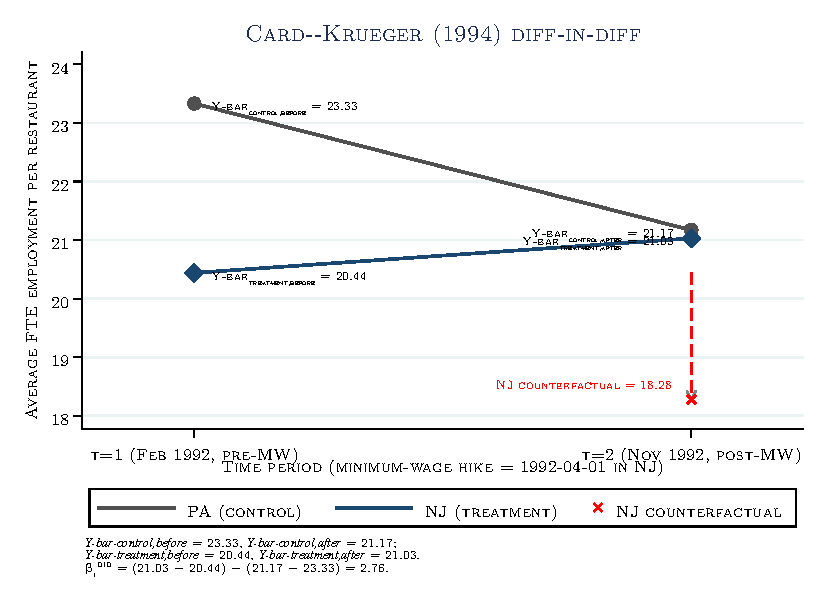
\includegraphics[width=0.95\textwidth]{output/figures/prob2_did_fig.pdf}
\caption{Card and Krueger (1994) difference-in-differences graphic. The solid navy line connects New Jersey's pre-period mean FTE employment ($20.44$) to its post-period mean ($21.03$); the solid gray line connects Pennsylvania's pre- ($23.33$) and post-period ($21.17$) means. Under the parallel-trends assumption, the NJ counterfactual-after mean (red ``X'' at $18.28$) equals NJ-before $+$ (PA-after $-$ PA-before). The DiD estimator $\hat{\beta}_1^{\textit{diffs-in-diffs}} = 0.59 - (-2.16) = 2.75$ (or $2.76$ in the authors' more-precise microdata) is the vertical distance from the red X to the actual NJ-after point.}
\label{fig:p2-did}
\end{figure}

\newpage

\section*{Replication Files}
\addcontentsline{toc}{section}{Replication Files}

All replication materials for \texttt{homework\_07} are available on GitHub:

\begin{itemize}
    \item Course repository: \url{https://github.com/tylersotomayor/econun3412-spring2026}
    \item Homework 07 folder: \url{https://github.com/tylersotomayor/econun3412-spring2026/tree/main/homework_07}
\end{itemize}

The \texttt{do\_files/} subfolder contains \texttt{ps7\_ajr.do}, \texttt{ps7\_sw\_ee.do}, and \texttt{ps7\_diff\_fig.do}. Each script writes a matching \texttt{.log} file. The \texttt{output/} subfolder stores the generated tables and figures used in this document.

\newpage
\bibliographystyle{apalike}
\bibliography{references}

\end{document}
